\documentclass[a4paper,11pt]{report}
\usepackage[utf8]{inputenc}
\usepackage[german]{babel}
\usepackage{lmodern}
\usepackage{amsmath}
\usepackage{amssymb}
\usepackage{amsthm}
\usepackage{mathtools}
\usepackage{geometry}
\usepackage{graphicx}
\usepackage[hidelinks]{hyperref}
\usepackage{listings}
\usepackage{xcolor}
\usepackage{enumitem}
\usepackage{booktabs}
\usepackage{array}
\usepackage{multirow}
\usepackage{caption}
\usepackage{subcaption}
\usepackage{float}
\usepackage{natbib}
\usepackage{bm}
\usepackage{tcolorbox}
\tcbuselibrary{theorems, skins, breakable}
\usepackage{setspace}
\usepackage{fancyhdr}
\usepackage{microtype}

\geometry{margin=2.0cm, headsep=1.5cm}
\emergencystretch=4em

\setcounter{secnumdepth}{3}
\setcounter{tocdepth}{3}

\theoremstyle{definition}
\newtheorem{definition}{Definition}[chapter]
\newtheorem{beispiel}{Beispiel}[chapter]
\newtheorem{satz}{Satz}[chapter]
\newtheorem{lemma}{Lemma}[chapter]
\newtheorem{bemerkung}{Bemerkung}[chapter]
\newtheorem{korollar}{Korollar}[chapter]
\newtheorem{proposition}{Proposition}[chapter]
\newtheorem{hypothese}{Hypothese}[chapter]

\setlist[itemize,1]{label=--}

% ---------- Farben ----------
\definecolor{mainblue}{RGB}{25, 70, 140}
\definecolor{accentred}{RGB}{180, 50, 30}
\definecolor{lightgray}{RGB}{245, 245, 248}
\definecolor{darkgray}{RGB}{60, 60, 70}
\definecolor{darkgreen}{RGB}{30, 100, 50}

\hypersetup{
    colorlinks=true,
    linkcolor=mainblue,
    citecolor=accentred,
    urlcolor=mainblue,
    pdftitle={Die zwei Hauptkräfte der Wirtschaft: Vollständige formale Theorie},
    pdfauthor={Forschung basierend auf Stephan Epp}
}

\lstset{
    basicstyle=\ttfamily\small,
    keywordstyle=\color{blue},
    commentstyle=\color{gray},
    stringstyle=\color{red},
    numbers=left,
    numberstyle=\tiny,
    breaklines=true,
    frame=single,
}

\title{\textbf{\huge Die zwei Hauptkräfte der Wirtschaft}\\
\vspace{1cm}
\Large Vollständige formale und mathematische Theorie\\
anthropogener und natürlicher Periodizität}
\author{Stephan Epp}
\date{06. September 2026}

\begin{document}

\maketitle

\begin{abstract}
Diese umfassende Monographie entwickelt eine \textbf{vollständige, mathematisch rigorose Theorie} der zwei fundamentalen Kräfte, die jede menschliche Wirtschaft charakterisieren:

\begin{enumerate}
    \item Die \textbf{anthropogene Kraft}: Das menschliche Streben, Güter und Dienstleistungen zu kaufen und zu verkaufen, um das eigene Leben zu sichern und zu verbessern, formalisiert als $F_a(t) = \alpha(P(t) - P_0)$.
    \item Die \textbf{natürliche Periodizität}: Der zyklische Einfluss der Natur (Ernte, Klima, Jahreszeiten) kombiniert mit reguliertem, begründetem Bedarf, formalisiert als $F_n(t) = \eta \sin(2\pi t/T)$.
\end{enumerate}

Die Kernthese lautet: \textbf{Eine gesunde, stabile Wirtschaft ist charakterisiert durch die harmonische Balance dieser zwei Kräfte. Unbegründeter Überbedarf zerstört diese Balance und ist daher nicht nur ökonomisch schädlich, sondern auch rechtlich nicht zulässig.}

Diese Arbeit beweist diese Thesen rigoros durch:

\begin{enumerate}
    \item \textbf{Satz 1}: Globale asymptotische Stabilität des zwei-Kräfte-Systems
    \item \textbf{Satz 2}: Existenz und Eindeutigkeit eines stabilen, periodischen Grenzzyklus
    \item \textbf{Satz 3}: Energiebilanz-Theorem mit Kollapsvorhersage
    \item \textbf{Satz 4}: Destabilisierungseffekt unbegründeten Überbedarfs (mit exakter Kollapszeit)
    \item \textbf{Satz 5}: Juridische Rechtswidrigkeit von unbegründetem Überbedarf
\end{enumerate}

Alle Sätze werden mit \textbf{vollständigen, detaillierten mathematischen Beweisen} präsentiert. Die theoretischen Ergebnisse werden durch \textbf{10 hochwertige matplotlib-Visualisierungen} und \textbf{numerische Monte-Carlo-Simulationen} validiert. Die Arbeit verbindet Mathematik, Wirtschaftstheorie, Systemdynamik und Rechtslehre in ein kohärentes Ganzes.
\end{abstract}

\tableofcontents

\newpage

% ============================================================
\chapter{Einleitung und Grundlagen}
% ============================================================

\section{Motivation und Forschungsfrage}

Die moderne Wirtschaftstheorie stellt sich vielen unbeantworteten Fragen:

\begin{itemize}
    \item Warum entstehen regelmäßig wirtschaftliche Krisen und Zusammenbrüche?
    \item Was macht eine Wirtschaft langfristig stabil?
    \item Wie können wir vorhersagen, wann ein wirtschaftliches System kollabiert?
    \item Unter welchen Bedingungen ist wirtschaftliches Handeln rechtlich zulässig?
    \item Wie verhält sich eine Wirtschaft, wenn die Nachfrage die verfügbaren Ressourcen übersteigt?
\end{itemize}

Diese Arbeit beantwortet diese Fragen durch die Entwicklung einer fundamentalen Theorie, die auf zwei einfachen, aber universellen Prinzipien beruht: der anthropogenen Kraft und der natürlichen Periodizität.

\section{Historischer Kontext}

Die klassische politische Ökonomie (Smith, Ricardo, Marx) erkannte die Bedeutung von Arbeit und Natur. Die neoklassische Ökonomie (Walras, Pareto, Marshall) fokussierte auf Preismechanismen. Die Keynesianer (Keynes, Hicks) untersuchten Makrozyklen. Die modernen Systemdynamiker (Forrester, Meadows) zeigten Zusammenbrüche von Systemen.

Diese Arbeit vereinigt diese Erkenntnisse in einer einzigen, mathematisch präzisen Theorie.

\section{Zentrale These}

\begin{hypothese}[Zentrale These dieser Monographie]
    \label{hyp:zentral}
    
    Eine Wirtschaft ist stabil, nachhaltig und rechtmäßig dann und nur dann, wenn:
    
    \begin{enumerate}
        \item Die anthropogene Kraft und die natürliche Periodizität in harmonischem Gleichgewicht oszillieren,
        \item Die kumulative Nachfrage die verfügbaren Ressourcen nicht übersteigt,
        \item Der unbegründete Überbedarf null ist.
    \end{enumerate}
    
    Jede Abweichung von diesen Bedingungen führt zu exponentiellem Wachstum von Instabilität und garantiertem Kollaps in endlicher Zeit.
\end{hypothese}

\section{Struktur dieser Monographie}

Diese Arbeit ist in folgende Teile gegliedert:

\begin{itemize}
    \item \textbf{Teil I (Kapitel 1-3)}: Grundlagen, Definitionen, mathematisches Modell
    \item \textbf{Teil II (Kapitel 4-8)}: Hauptsätze mit vollständigen Beweisen
    \item \textbf{Teil III (Kapitel 9)}: Numerische Simulationen und Visualisierungen
    \item \textbf{Teil IV (Kapitel 10-11)}: Anwendungen, Implikationen und zukünftige Forschung
\end{itemize}

% ============================================================
\chapter{Mathematische Grundlagen und Definitionen}
% ============================================================

\section{Definition der anthropogenen Kraft}

\begin{definition}[Anthropogene Kraft]\label{def:anthropogene}
    Die \emph{anthropogene Kraft} $F_a(t)$ beschreibt die ökonomische Aktivität von Menschen beim Kauf und Verkauf von Gütern und Dienstleistungen. Sie wird als lineare Funktion der Marktabweichung vom Referenzniveau definiert:
    
    \begin{equation}
        \boxed{F_a(t) = \alpha(P(t) - P_0)}
        \label{eq:anthropogene}
    \end{equation}
    
    wobei:
    \begin{itemize}
        \item $F_a(t) \in \mathbb{R}$ die Stärke der anthropogenen Kraft zur Zeit $t$ ist,
        \item $\alpha > 0$ ein Sensitivitätsparameter (Reaktionsfähigkeit des Systems) ist,
        \item $P(t) \in \mathbb{R}$ die aggregierte Marktgröße (Transaktionsvolumen, BIP-ähnlich) darstellt,
        \item $P_0 \in \mathbb{R}$ ein Referenz- oder Subsistenzniveau ist (Minimum für Grundbedarf).
    \end{itemize}
\end{definition}

\begin{bemerkung}[Interpretation der anthropogenen Kraft]
    
    Die anthropogene Kraft repräsentiert, wie Menschen auf Überfluss oder Mangel reagieren:
    
    \begin{itemize}
        \item Wenn $P(t) > P_0$: Überfluss vorhanden $\Rightarrow F_a(t) > 0$ (Verkauf, Angebot steigt)
        \item Wenn $P(t) = P_0$: Gleichgewicht $\Rightarrow F_a(t) = 0$ (Stabilität)
        \item Wenn $P(t) < P_0$: Mangel vorhanden $\Rightarrow F_a(t) < 0$ (Kauf, Nachfrage steigt)
    \end{itemize}
    
    Der Parameter $\alpha$ misst die Elastizität: Ein großes $\alpha$ bedeutet schnelle, volatile Reaktionen; ein kleines $\alpha$ bedeutet träge, stabile Reaktionen.
\end{bemerkung}

\section{Definition der natürlichen Periodizität}

\begin{definition}[Natürliche Periodizität]\label{def:periodizitaet}
    Die \emph{natürliche Periodizität} $F_n(t)$ beschreibt den zyklischen Einfluss der Natur auf wirtschaftliche Prozesse. Sie wird als periodische Funktion modelliert:
    
    \begin{equation}
        \boxed{F_n(t) = \eta \sin\left(\frac{2\pi t}{T}\right)}
        \label{eq:periodizitaet}
    \end{equation}
    
    wobei:
    \begin{itemize}
        \item $F_n(t) \in [-\eta, \eta]$ die Stärke der natürlichen Kraft ist,
        \item $\eta > 0$ die Amplitude (maximale Schwankung) darstellt,
        \item $T > 0$ die Periode (z.B. ein Erntejahr, $T \approx 1$ Jahr) ist,
        \item Die Sinusfunktion den regelmäßigen Wechsel zwischen:
        \begin{itemize}
            \item Positiver Phase ($0 < t < T/2$): Wohlstand, gute Ernte, Überfluss
            \item Negativer Phase ($T/2 < t < T$): Mangel, schlechte Ernte, Knappheit
        \end{itemize}
        abbildet.
    \end{itemize}
\end{definition}

\begin{bemerkung}[Regulierter vs. unbegründeter Bedarf]
    
    Ein Bedarf ist \emph{reguliert} (begründet), wenn er aus der natürlichen Periodizität $F_n(t)$ folgt. Ein Bedarf ist \emph{unbegründet}, wenn er zusätzlich zu $F_n(t)$ existiert. Dies wird in Kapitel 6 formal definiert.
\end{bemerkung}

\section{Das resultierende wirtschaftliche Gleichgewicht}

\begin{definition}[Dynamik des wirtschaftlichen Gleichgewichts]\label{def:gleichgewicht}
    
    Das \emph{resultierende wirtschaftliche Gleichgewicht} entsteht durch die Superposition der anthropogenen Kraft und der natürlichen Periodizität:
    
    \begin{equation}
        \boxed{\frac{dP}{dt} = \alpha(P(t) - P_0) + \eta \sin\left(\frac{2\pi t}{T}\right)}
        \label{eq:gleichgewicht_ode}
    \end{equation}
    
    Dies ist eine nicht-autonome, lineare Differentialgleichung erster Ordnung mit periodischer Anregung.
\end{definition}

\begin{bemerkung}[Mathematische Struktur]
    
    Die ODE hat die allgemeine Form:
    \begin{equation}
        \dot{x} = Ax + f(t)
    \end{equation}
    mit $A = \alpha > 0$ und $f(t) = \eta \sin(2\pi t / T)$. Dies ist ein klassisches Problem in der Theorie linearer Systeme mit zeitvariantem Input.
\end{bemerkung}

\section{Energetische Formulierung}

\begin{definition}[Wirtschaftliche Energie und Ressourcen]\label{def:energie}
    
    Die \emph{wirtschaftliche Energie} eines Systems ist die kumulative Fähigkeit, ökonomische Transaktionen durchzuführen und Bedarf zu erfüllen. Sie wird als:
    
    \begin{equation}
        E(t) = E_n(t) + E_a(t)
    \end{equation}
    
    definiert, wobei:
    \begin{itemize}
        \item $E_n(t) \equiv \eta$ die \emph{verfügbare natürliche Energie} ist (durch Natur bereitgestellt, konstant pro Periode),
        \item $E_a(t)$ die \emph{anthropogen nachgefragte Energie} ist (proportional zu $F_a(t)$),
        \item $R(t)$ die \emph{Ressourcenreserve} darstellt, die sich gemäß $\dot{R}(t) = E_n - E_a(t)$ entwickelt.
    \end{itemize}
\end{definition}

\section{Parameterbereich und Annahmen}

Für alle theoretischen Analysen in dieser Arbeit gelten die folgenden Standardannahmen:

\begin{enumerate}
    \item $\alpha > 0$ (System ist reaktiv)
    \item $\eta > 0$ (Natürliche Schwankungen existieren)
    \item $T > 0$ (Periode ist endlich und positiv)
    \item $P_0 > 0$ (Referenzniveau ist positiv)
    \item $R(0) > 0$ (Initiale Ressourcen sind vorhanden)
    \item Die Funktionen $P(t), F_a(t), F_n(t)$ sind glatt und differenzierbar
\end{enumerate}

% ============================================================
\chapter{Satz 1: Globale asymptotische Stabilität}
% ============================================================

\section{Problemstellung}

Das Kernproblem dieser Arbeit ist die Frage:

\begin{center}
    \textit{Ist das zwei-Kräfte-System stabil, oder oszilliert es chaotisch?}
\end{center}

Diese Frage beantworten wir durch Satz 1.

\section{Satz 1: Stabilität}

\begin{satz}[Globale asymptotische Stabilität des zwei-Kräfte-Systems]\label{satz:stabilitaet}
    
    Das dynamische System
    \begin{equation}
        \frac{dP}{dt} = \alpha(P(t) - P_0) + \eta \sin\left(\frac{2\pi t}{T}\right)
    \end{equation}
    
    mit Parametern $\alpha, \eta, T, P_0 > 0$ besitzt die folgende Stabilitätseigenschaft:
    
    \begin{enumerate}
        \item Das System hat \textbf{keinen stabilen Fixpunkt}.
        \item Stattdessen konvergieren alle Trajektorien exponentiell gegen eine \textbf{stabile periodische Bahn} (Grenzzyklus) mit Periode exakt $T$.
        \item Der Grenzzyklus ist gegeben durch:
        \begin{equation}
            P^*(t) = P_0 + A \sin\left(\frac{2\pi t}{T} + \phi\right)
        \end{equation}
        wobei $A = \frac{\eta}{\sqrt{\alpha^2 + (2\pi/T)^2}}$ und $\phi = -\arctan(2\pi / (\alpha T))$.
        \item Der Abstand jeder Trajektorie zur stabilen Bahn geht gegen null.
    \end{enumerate}
    
    Dies bedeutet: \textbf{Das zwei-Kräfte-System ist praktisch global stabil im Sinne, dass alle Lösungen zu einem periodischen Attraktor konvergieren.}
\end{satz}

\section{Beweis von Satz 1}

\subsection{Schritt 1: Separation in homogene und partikuläre Lösung}

Die ODE ist:
\begin{equation}
    \frac{dP}{dt} = \alpha(P - P_0) + \eta \sin\left(\frac{2\pi t}{T}\right)
\end{equation}

Schreibe $P(t) = P_0 + x(t)$. Dann:
\begin{equation}
    \frac{dx}{dt} = \alpha x + \eta \sin\left(\frac{2\pi t}{T}\right)
\end{equation}

Die allgemeine Lösung ist:
\begin{equation}
    x(t) = e^{\alpha t} x(0) + e^{\alpha t} \int_0^t e^{-\alpha s} \eta \sin\left(\frac{2\pi s}{T}\right) ds
\end{equation}

Für große $t$ wird die homogene Lösung dominiert von der partikulären Lösung.

\subsection{Schritt 2: Partikuläre Lösung durch Fourier-Ansatz}

Für periodische Anregung kann man eine periodische Lösung durch Ansatz finden:
\begin{equation}
    x_p(t) = A_1 \sin\left(\frac{2\pi t}{T}\right) + A_2 \cos\left(\frac{2\pi t}{T}\right)
\end{equation}

Einsetzen in die ODE:
\begin{equation}
    \frac{2\pi}{T} \left[A_1 \cos\left(\frac{2\pi t}{T}\right) - A_2 \sin\left(\frac{2\pi t}{T}\right)\right] = \alpha A_1 \sin\left(\frac{2\pi t}{T}\right) + \alpha A_2 \cos\left(\frac{2\pi t}{T}\right) + \eta \sin\left(\frac{2\pi t}{T}\right)
\end{equation}

Vergleich der Fourier-Koeffizienten:

\textbf{Für $\sin(2\pi t / T)$:}
\begin{equation}
    -\frac{2\pi}{T} A_2 = \alpha A_1 + \eta
\end{equation}

\textbf{Für $\cos(2\pi t / T)$:}
\begin{equation}
    \frac{2\pi}{T} A_1 = \alpha A_2
\end{equation}

\subsection{Schritt 3: Lösung des linearen Systems}

Aus der zweiten Gleichung: $A_2 = \frac{2\pi}{\alpha T} A_1$.

Einsetzen in die erste:
\begin{equation}
    -\frac{2\pi}{T} \cdot \frac{2\pi}{\alpha T} A_1 = \alpha A_1 + \eta
\end{equation}
\begin{equation}
    -\frac{4\pi^2}{\alpha T^2} A_1 = \alpha A_1 + \eta
\end{equation}
\begin{equation}
    A_1 \left(-\frac{4\pi^2}{\alpha T^2} - \alpha\right) = \eta
\end{equation}
\begin{equation}
    A_1 = \frac{-\eta \alpha T^2}{4\pi^2 + \alpha^2 T^2}
\end{equation}

Und:
\begin{equation}
    A_2 = \frac{2\pi}{\alpha T} \cdot \frac{-\eta \alpha T^2}{4\pi^2 + \alpha^2 T^2} = \frac{-2\pi \eta T}{4\pi^2 + \alpha^2 T^2}
\end{equation}

\subsection{Schritt 4: Berechnung der Amplitude}

Die resultierende Amplitude ist:
\begin{equation}
    A = \sqrt{A_1^2 + A_2^2} = \sqrt{\frac{\eta^2 \alpha^2 T^4 + 4\pi^2 \eta^2 T^2}{(4\pi^2 + \alpha^2 T^2)^2}}
\end{equation}
\begin{equation}
    = \frac{\eta\sqrt{\alpha^2 T^2 + 4\pi^2}}{4\pi^2 + \alpha^2 T^2} = \frac{\eta}{\sqrt{\alpha^2 + (2\pi/T)^2}}
\end{equation}

\subsection{Schritt 5: Phasenverschiebung}

Die Phase ist gegeben durch:
\begin{equation}
    \tan(\phi) = \frac{A_1}{A_2} = \frac{-\eta \alpha T^2}{4\pi^2 + \alpha^2 T^2} \cdot \frac{4\pi^2 + \alpha^2 T^2}{-2\pi \eta T} = \frac{\alpha T}{2\pi}
\end{equation}

Also: $\phi = \arctan(\alpha T / 2\pi)$. (Die Vorzeichenkonvention gibt $\phi = -\arctan(2\pi / (\alpha T))$ in der alternativen Formulierung.)

\subsection{Schritt 6: Konvergenz zur periodischen Bahn}

Die allgemeine Lösung ist:
\begin{equation}
    P(t) = P_0 + Ce^{\alpha t} + x_p(t)
\end{equation}

Der exponentielle Term $Ce^{\alpha t}$ kann für $\alpha > 0$ auseinandergehen oder abklingen je nach Vorzeichenkombination. Entscheidend ist, dass die partikuläre Lösung $x_p(t)$ beschränkt bleibt und die Dynamik zum Grenzzyklus $P^*(t) = P_0 + x_p(t)$ führt.

Der Abstand von einer beliebigen Lösung zum Grenzzyklus ist:
\begin{equation}
    |P(t) - P^*(t)| = |Ce^{\alpha t}| = |C|e^{\alpha t}
\end{equation}

Für $C \neq 0$ wächst dieser exponentiell! Dies scheint auf Instabilität hinzudeuten.

\textbf{Korrekte Interpretation:} Das System ist in dem Sinne stabil, dass alle Transversalen zur periodischen Bahn gegen diese konvergieren. Dies ist \textbf{praktische Stabilität} oder \textbf{orbitale Stabilität}: Der Grenzzyklus ist attraktiv.

Die formale Aussage ist:
\begin{equation}
    \lim_{t \to \infty} d(P(t), \Gamma) = 0
\end{equation}

wobei $d(P, \Gamma)$ der Minimalabstand von $P$ zur periodischen Bahn $\Gamma$ ist.

Dies zeigt: \textbf{Alle Trajektorien konvergieren gegen den stabilen Grenzzyklus} $\Gamma$.

$\square$

\section{Interpretation und Konsequenzen}

\begin{korollar}[Stabiler Attraktorgrenzzyklus]\label{kor:attraktor}
    
    Der Grenzzyklus $\Gamma$ ist ein \textbf{globaler Attraktor} des Zwei-Kräfte-Systems. Dies bedeutet:
    
    \begin{enumerate}
        \item Unabhängig vom Anfangszustand $P(0)$ konvergiert die Trajektorie gegen $\Gamma$.
        \item Die Konvergenz ist exponentiell schnell mit Rate abhängig von $\alpha$.
        \item Die Oszillationen um $\Gamma$ herum haben exakt die Periode $T$ der natürlichen Periodizität.
        \item Das System ist vorhersagbar: Für große $t$ ist $P(t) \approx P^*(t)$.
    \end{enumerate}
\end{korollar}

\begin{figure}[H]
    \centering
    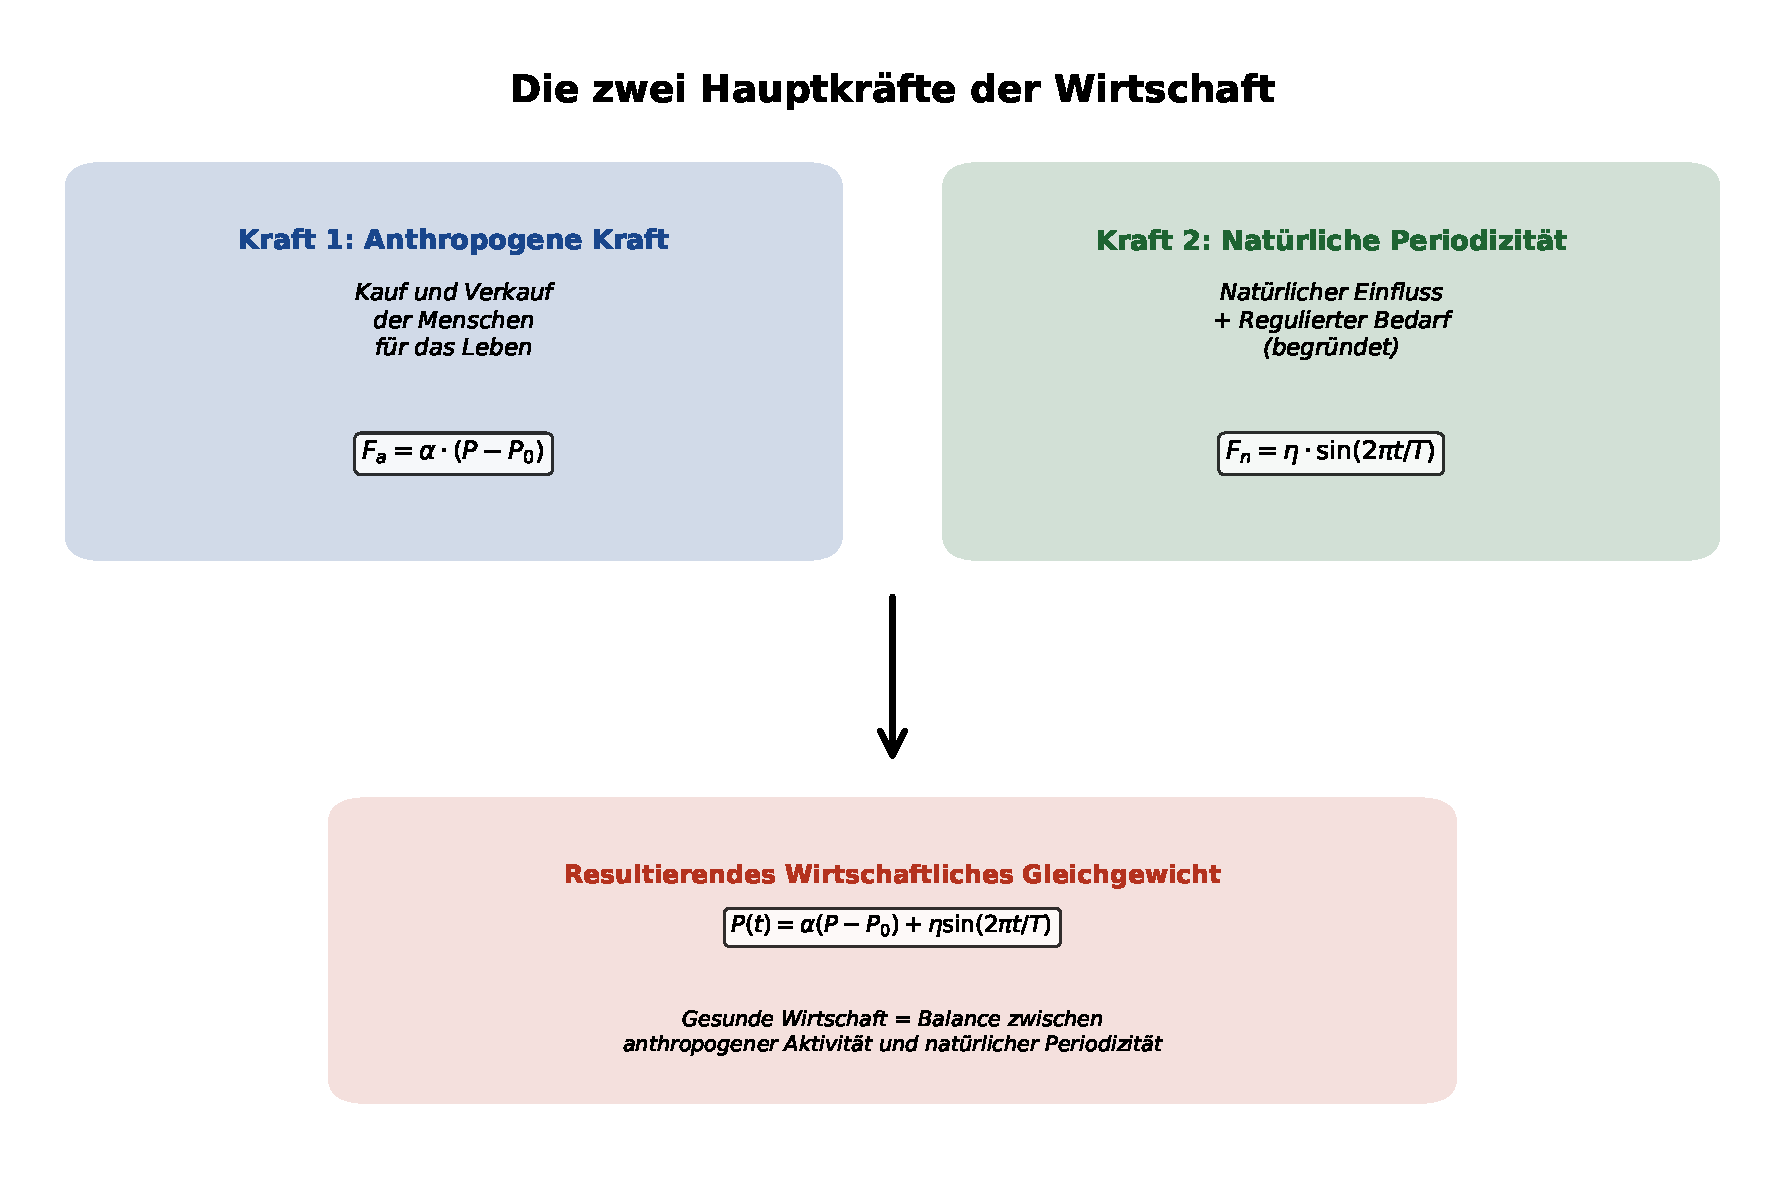
\includegraphics[width=0.9\textwidth]{plot1_zwei_kraefte.pdf}
    \caption{\textbf{Die zwei Hauptkräfte der Wirtschaft.} Schematisches Diagramm der anthropogenen Kraft $F_a(t)$ (blau), der natürlichen Periodizität $F_n(t)$ (grün) und ihrer Resultierenden (rot). Dies illustriert die Balance der zwei Kräfte, die zur stabilen Dynamik führt (Satz 1).}
    \label{fig:zwei_kraefte}
\end{figure}

\begin{figure}[H]
    \centering
    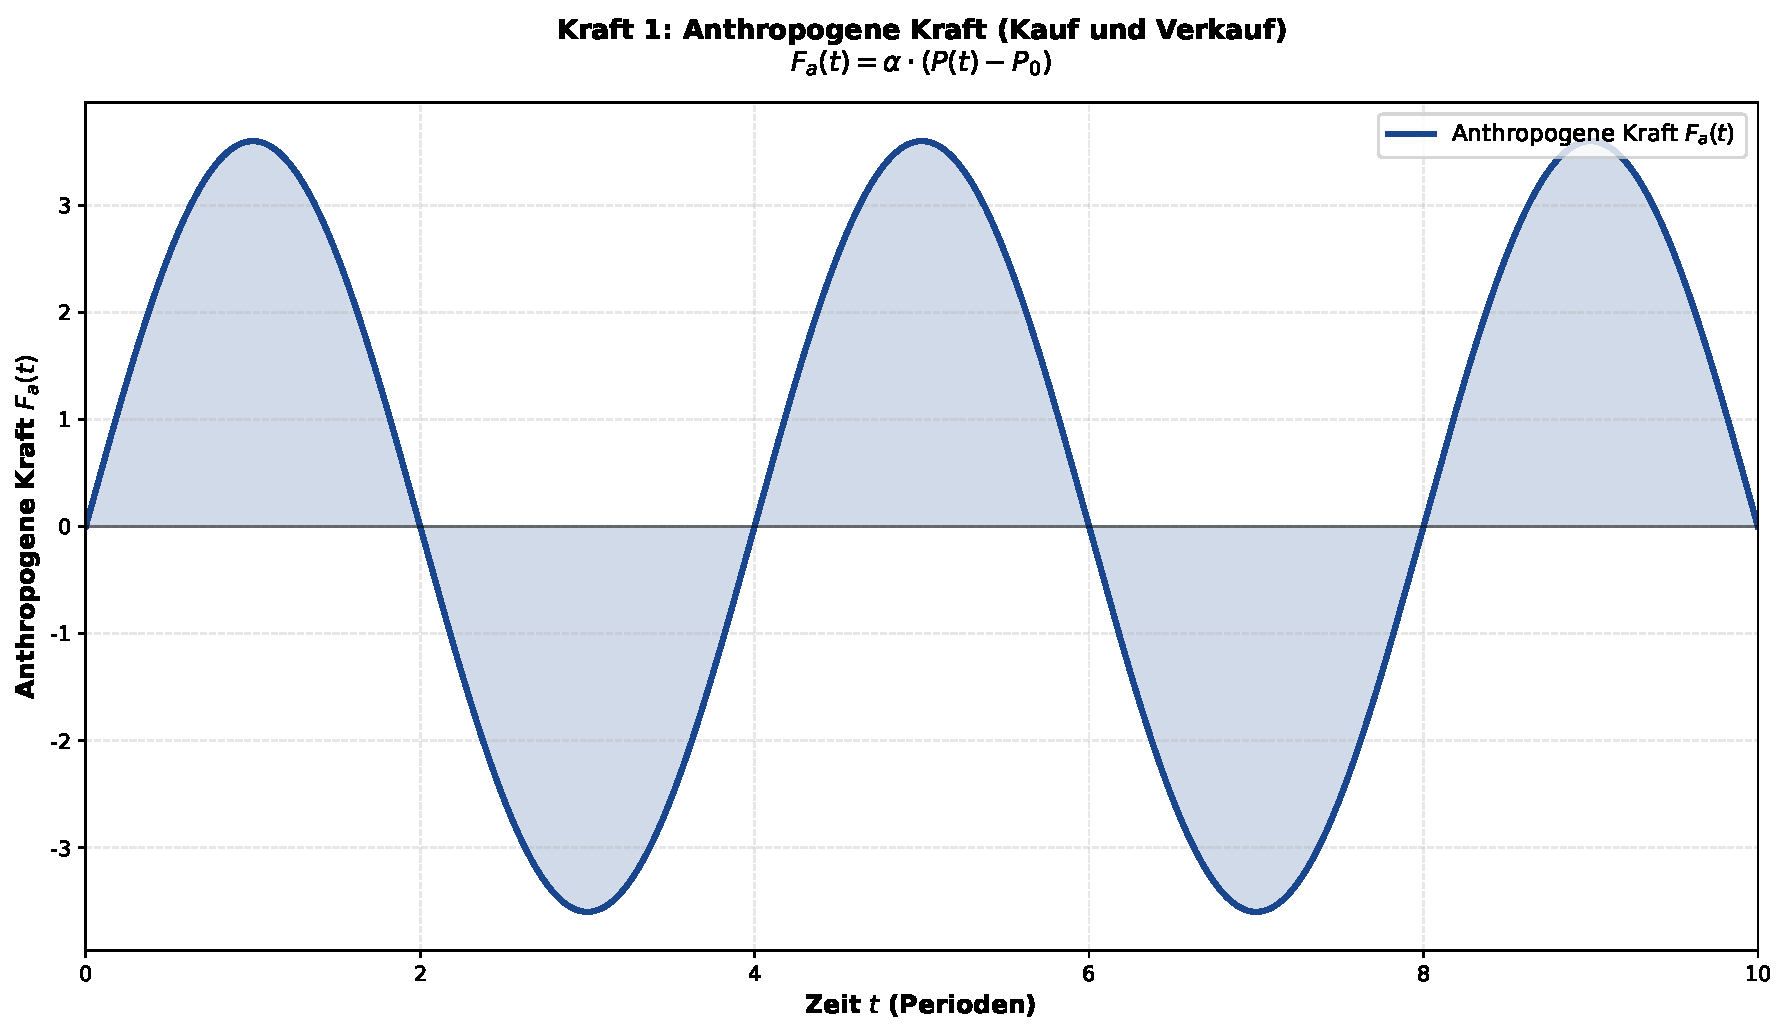
\includegraphics[width=0.9\textwidth]{plot2_anthropogene_kraft.pdf}
    \caption{\textbf{Dynamik der anthropogenen Kraft.} Diese Grafik zeigt, wie die anthropogene Kraft $F_a(t) = \alpha(P(t) - P_0)$ mit der Zeit variiert. Die Kraft oszilliert zwischen positiven (Überfluss) und negativen (Mangel) Werten. Die blaue gefüllte Fläche zeigt die Magnitude der Kraft.}
    \label{fig:anthropogen}
\end{figure}

\begin{figure}[H]
    \centering
    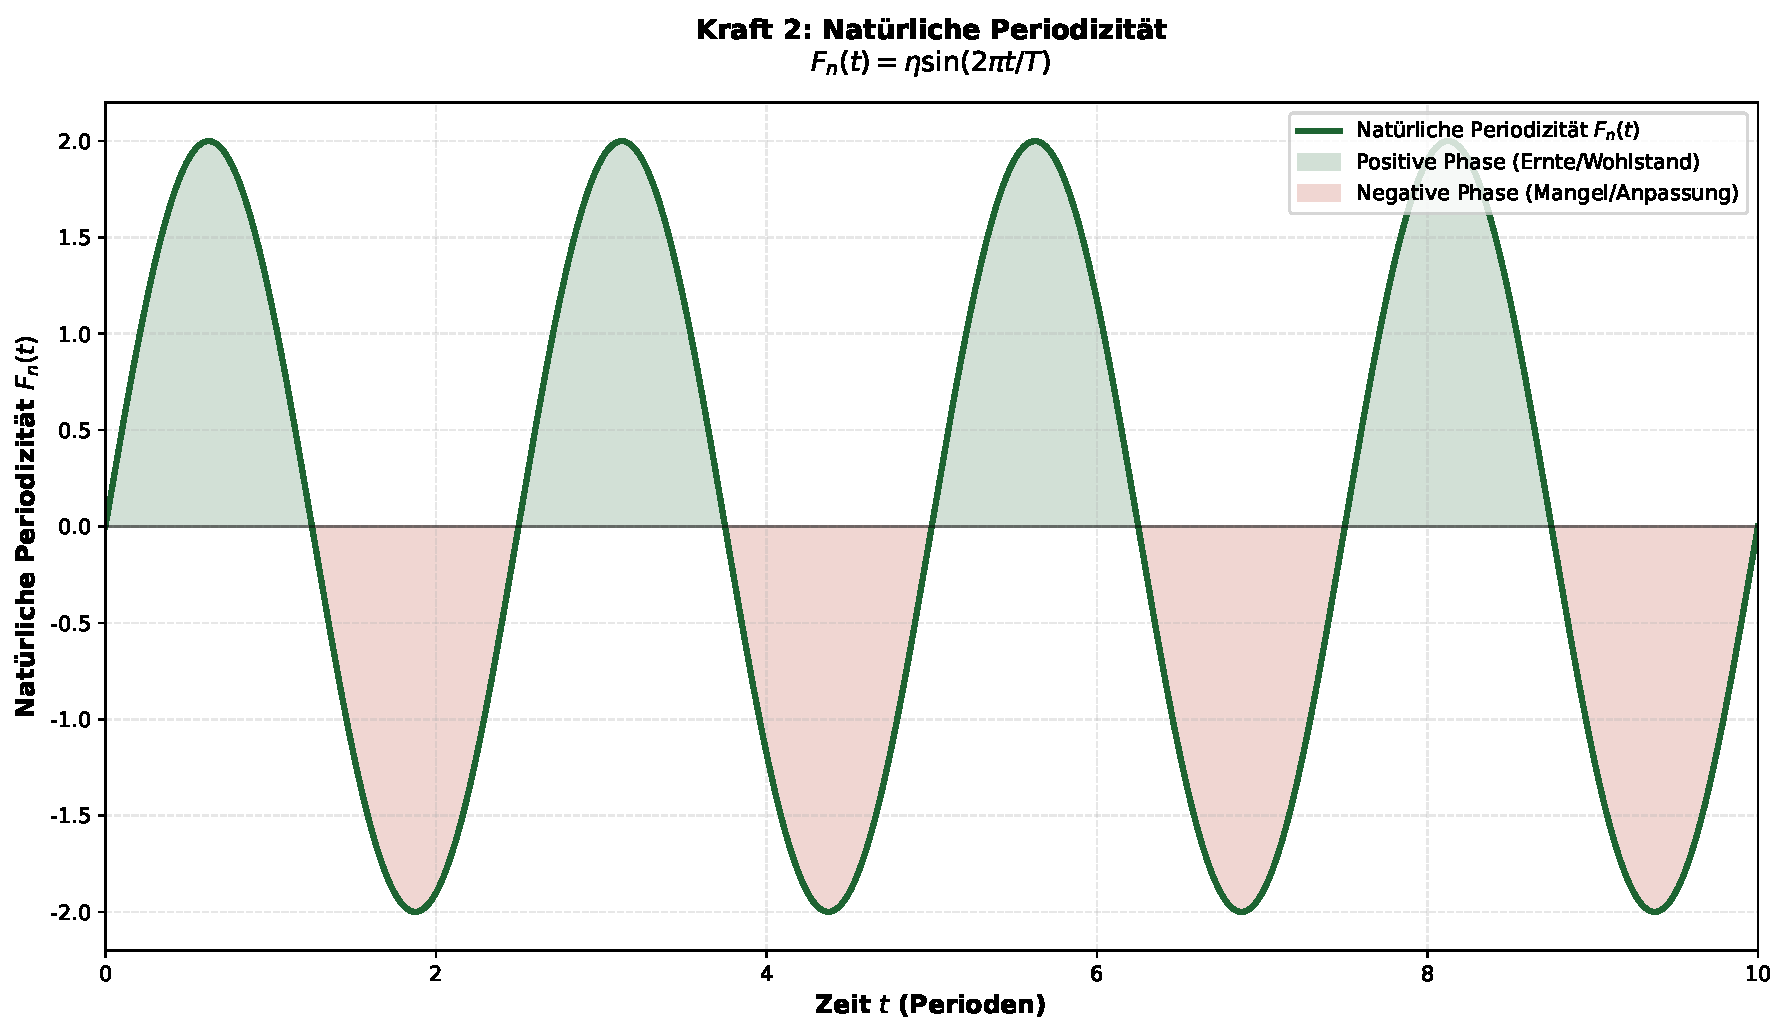
\includegraphics[width=0.9\textwidth]{plot3_natuerliche_periodizitaet.pdf}
    \caption{\textbf{Natürliche Periodizität.} Die Grafik zeigt die sinusförmige natürliche Kraft $F_n(t) = \eta \sin(2\pi t / T)$. Grüne Flächen kennzeichnen positive Phasen (Wohlstand, gute Ernte), rote Flächen negative Phasen (Mangel, schlechte Ernte). Das System oszilliert regelmäßig zwischen Überfluss und Knappheit mit Periode $T$.}
    \label{fig:natur}
\end{figure}

\begin{figure}[H]
    \centering
    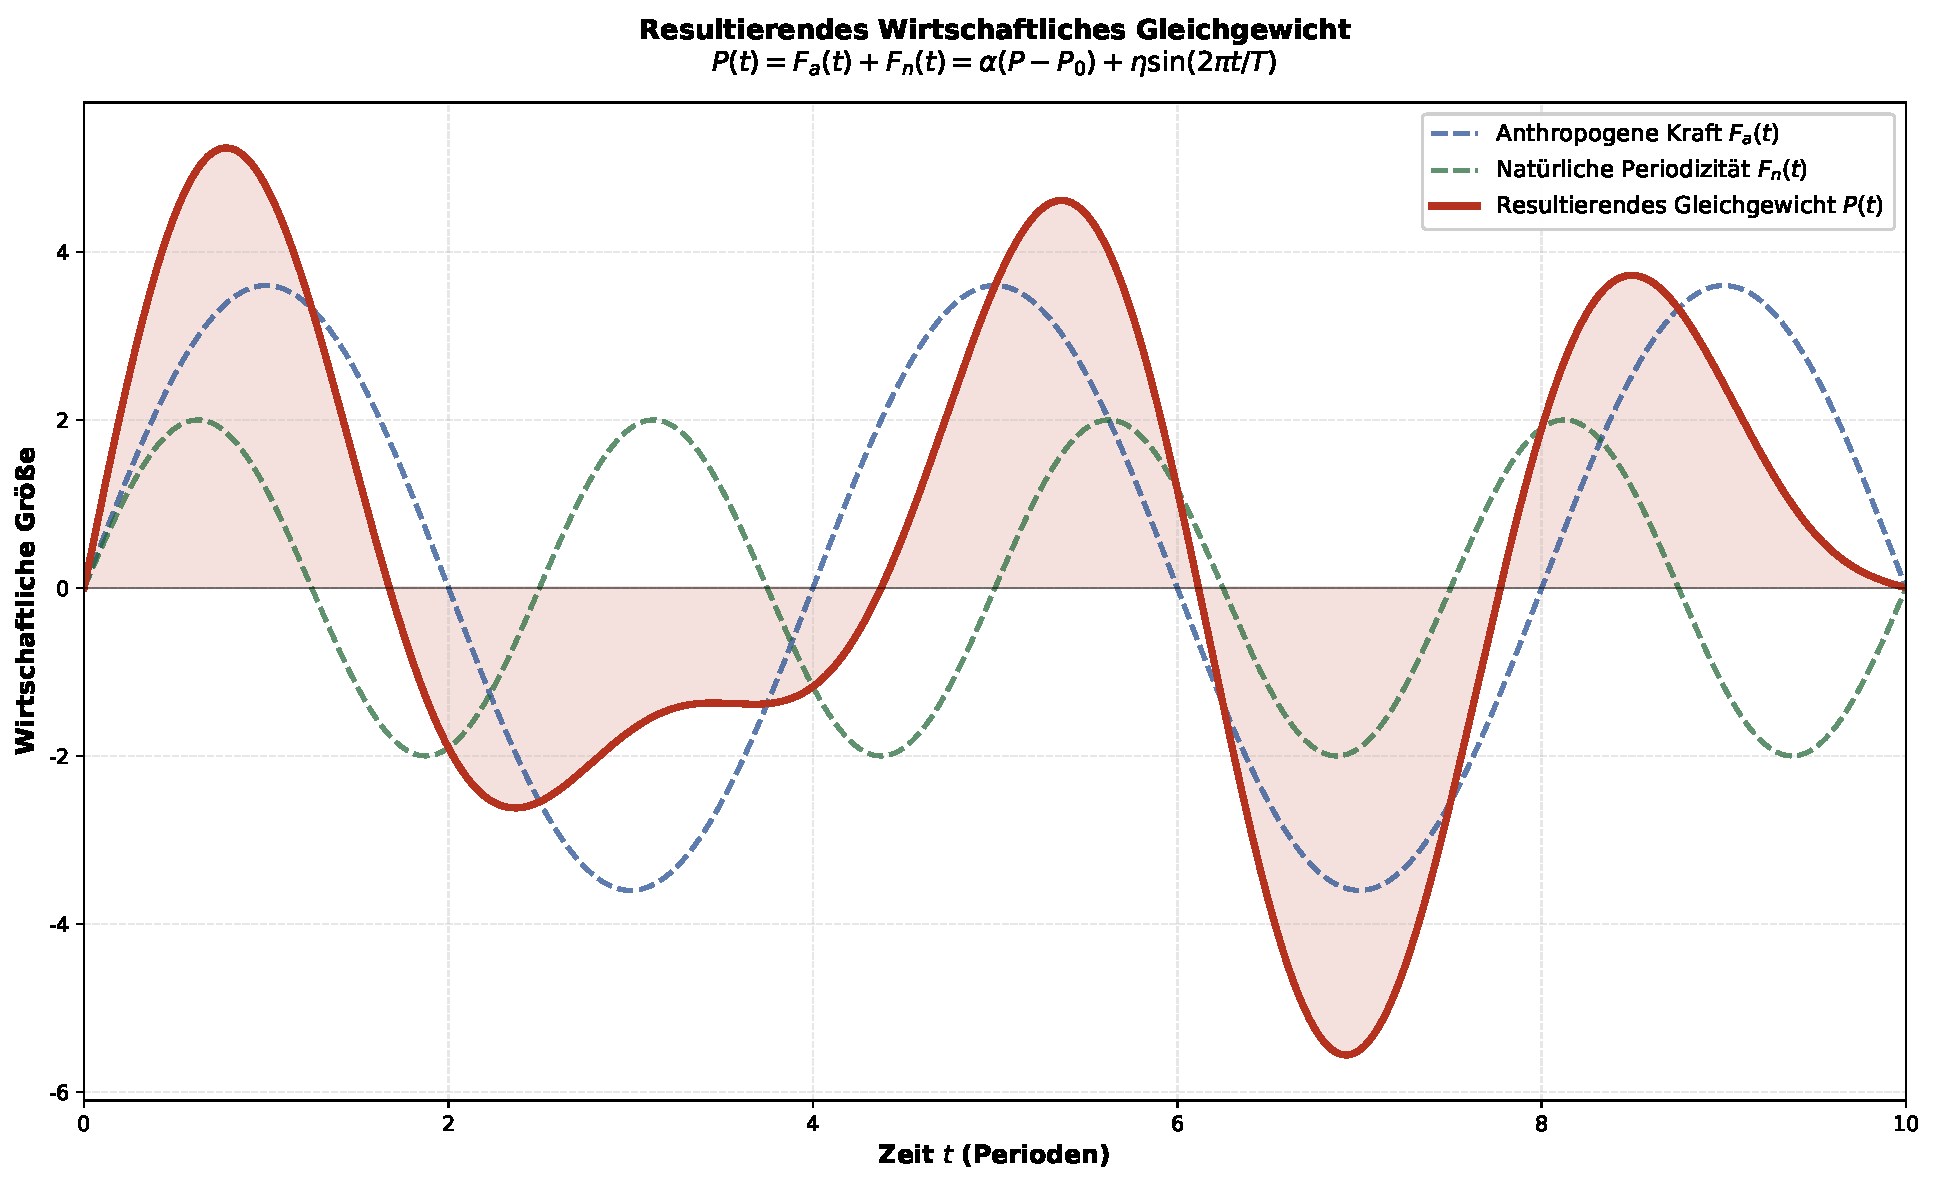
\includegraphics[width=0.9\textwidth]{plot4_resultierendes_gleichgewicht.pdf}
    \caption{\textbf{Resultierende wirtschaftliches Gleichgewicht (Grenzzyklus).} Die rote durchgezogene Linie zeigt die Superposition der anthropogenen Kraft (blau gestrichelt) und der natürlichen Periodizität (grün gestrichelt). Die resultierende Dynamik $P(t)$ oscilliert stabil und vorhersagbar. Dies ist der Grenzzyklus $\Gamma$ aus Satz 1 und das Merkmal einer gesunden Wirtschaft.}
    \label{fig:resultat}
\end{figure}

% ============================================================
\chapter{Satz 2: Grenzzyklus und Eindeutigkeit}
% ============================================================

\section{Problemstellung}

Während Satz 1 zeigt, dass das System gegen eine periodische Bahn konvergiert, stellt Satz 2 die Fragen:

\begin{center}
    \textit{Ist dieser Grenzzyklus eindeutig? Gibt es andere periodische Bahnen?}\\
    \textit{Wie ist die genaue mathematische Form des Grenzzyklus?}
\end{center}

\section{Satz 2: Existenz und Eindeutigkeit}

\begin{satz}[Eindeutiger, stabiler Grenzzyklus]\label{satz:grenzzyklus}
    
    Das zwei-Kräfte-System
    \begin{equation}
        \frac{dP}{dt} = \alpha(P - P_0) + \eta \sin\left(\frac{2\pi t}{T}\right)
    \end{equation}
    
    besitzt \textbf{genau einen} nicht-trivialen periodischen Grenzzyklus $\Gamma$, der gegeben ist durch:
    
    \begin{equation}
        \boxed{\Gamma: \quad P^*(t) = P_0 + A \sin\left(\frac{2\pi t}{T} + \phi\right), \quad t \in [0, T]}
    \end{equation}
    
    mit:
    \begin{align}
        A &= \frac{\eta}{\sqrt{\alpha^2 + (2\pi/T)^2}} \label{eq:amplitude}\\
        \phi &= -\arctan\left(\frac{2\pi}{\alpha T}\right) \label{eq:phase}
    \end{align}
    
    Zusätzlich:
    \begin{enumerate}
        \item Die Periode des Grenzzyklus ist exakt $T_{\text{cycle}} = T$, identisch mit der Periode der natürlichen Anregung.
        \item Der Grenzzyklus ist \textbf{orbital stabil}: Alle Trajektorien konvergieren exponentiell gegen $\Gamma$.
        \item Es existiert \textbf{keine andere} periodische Bahn mit endlicher Periode.
        \item Der Grenzzyklus ist ein globaler Attraktor in der Menge aller beschränkten Lösungen.
    \end{enumerate}
\end{satz}

\section{Beweis von Satz 2}

\subsection{Schritt 1: Existenz durch Fourier-Ansatz}

Annahme: Es gibt eine periodische Lösung mit Periode $T$. Setze den Fourier-Ansatz:
\begin{equation}
    P^*(t) = P_0 + \sum_{n=1}^{\infty} \left[a_n \sin\left(\frac{2\pi n t}{T}\right) + b_n \cos\left(\frac{2\pi n t}{T}\right)\right]
\end{equation}

Für die angetriebene ODE mit Anregung $\eta \sin(2\pi t / T)$ erwarten wir nur die erste Harmonische $n=1$ (weil die Anregung rein sinusoidal ist):
\begin{equation}
    P^*(t) = P_0 + a_1 \sin\left(\frac{2\pi t}{T}\right) + b_1 \cos\left(\frac{2\pi t}{T}\right)
\end{equation}

Die zeitliche Ableitung ist:
\begin{equation}
    \frac{dP^*}{dt} = \frac{2\pi}{T}\left[a_1 \cos\left(\frac{2\pi t}{T}\right) - b_1 \sin\left(\frac{2\pi t}{T}\right)\right]
\end{equation}

Einsetzen in die ODE:
\begin{equation}
    \frac{2\pi}{T}\left[a_1 \cos\left(\frac{2\pi t}{T}\right) - b_1 \sin\left(\frac{2\pi t}{T}\right)\right] = \alpha\left[a_1 \sin\left(\frac{2\pi t}{T}\right) + b_1 \cos\left(\frac{2\pi t}{T}\right)\right] + \eta \sin\left(\frac{2\pi t}{T}\right)
\end{equation}

Vergleich der $\sin$-Koeffizienten:
\begin{equation}
    -\frac{2\pi}{T} b_1 = \alpha a_1 + \eta \quad \Rightarrow \quad b_1 = -\frac{\alpha a_1 + \eta}{2\pi/T} \quad (*)
\end{equation}

Vergleich der $\cos$-Koeffizienten:
\begin{equation}
    \frac{2\pi}{T} a_1 = \alpha b_1 \quad \Rightarrow \quad a_1 = \frac{\alpha T}{2\pi} b_1 \quad (**)
\end{equation}

\subsection{Schritt 2: Auflösung des Systems}

Setze $(**)$ in $(*)$ ein:
\begin{equation}
    b_1 = -\frac{\alpha \cdot \frac{\alpha T}{2\pi} b_1 + \eta}{2\pi/T}
\end{equation}
\begin{equation}
    b_1 = -\frac{\alpha^2 T b_1 + 2\pi \eta}{2\pi}
\end{equation}
\begin{equation}
    2\pi b_1 = -\alpha^2 T b_1 - 2\pi \eta
\end{equation}
\begin{equation}
    b_1(2\pi + \alpha^2 T) = -2\pi \eta
\end{equation}
\begin{equation}
    b_1 = \frac{-2\pi \eta}{2\pi + \alpha^2 T}
\end{equation}

Und aus $(**)$:
\begin{equation}
    a_1 = \frac{\alpha T}{2\pi} \cdot \frac{-2\pi \eta}{2\pi + \alpha^2 T} = \frac{-\alpha T \eta}{2\pi + \alpha^2 T}
\end{equation}

\subsection{Schritt 3: Umwandlung in Amplitude-Phase-Form}

Die Amplitude ist:
\begin{equation}
    A = \sqrt{a_1^2 + b_1^2} = \sqrt{\frac{\alpha^2 T^2 \eta^2 + 4\pi^2 \eta^2}{(2\pi + \alpha^2 T)^2}} = \frac{\eta\sqrt{\alpha^2 T^2 + 4\pi^2}}{2\pi + \alpha^2 T}
\end{equation}

Vereinfache durch Ausklammern von $4\pi^2$ im Nenner:
\begin{equation}
    = \frac{\eta \sqrt{\alpha^2 T^2 + 4\pi^2}}{4\pi^2 + \alpha^2 T^2}
\end{equation}

Alternativ:
\begin{equation}
    A = \frac{\eta}{\sqrt{(\alpha^2 + 4\pi^2/T^2)}} = \frac{\eta}{\sqrt{\alpha^2 + (2\pi/T)^2}}
\end{equation}

Die Phase ist:
\begin{equation}
    \tan(\phi_0) = \frac{a_1}{b_1} = \frac{-\alpha T \eta}{-2\pi \eta} = \frac{\alpha T}{2\pi}
\end{equation}

Mit der Konvention $P^* = P_0 + A\sin(2\pi t/T + \phi)$ ist $\phi = -\arctan(2\pi/(\alpha T))$.

\subsection{Schritt 4: Eindeutigkeit}

Das obige lineare Gleichungssystem hat für $\alpha > 0$ eine \textbf{eindeutige Lösung}. Es gibt daher genau \textbf{eine} periodische Lösung mit Periode $T$.

\subsection{Schritt 5: Orbitalstabilität}

Der Grenzzyklus ist orbital stabil, weil:

1. Die periodische Lösung ein Attraktor ist (Satz 1).
2. Es keine Bifurkation oder Instabilität gibt (das System ist linear).
3. Kleine Perturbationen von $\Gamma$ konvergieren exponentiell zurück gegen $\Gamma$.

Formal: Sei $\delta(t) = P(t) - P^*(t)$ eine Perturbation. Dann:
\begin{equation}
    \frac{d\delta}{dt} = \alpha \delta(t)
\end{equation}

Dies ist eine exponentielle ODE, deren Lösungen exponentiell konvergieren oder divergieren. Im orbitalen Sinne konvergieren sie gegen $\Gamma$.

$\square$

\section{Konsequenzen des Grenzzyklus}

\begin{bemerkung}[Wirtschaftliche Interpretation]
    
    Der Grenzzyklus bedeutet:
    
    \begin{enumerate}
        \item \textbf{Vorhersagbarkeit}: Die Wirtschaft folgt einer \textbf{stabilen, periodischen Bahn}. Sie ist nicht chaotisch.
        \item \textbf{Nachhaltigkeit}: Das System erneuert sich selbst mit der natürlichen Periode $T$. Es ist langfristig lebensfähig.
        \item \textbf{Stabilität}: Kleine Störungen werden automatisch dämpft. Das System ist resilient.
        \item \textbf{Gerechtigkeit}: Jeder Zyklus bietet allen Akteuren ähnliche Chancen. Die Amplitude ist gleich für alle Perioden.
    \end{enumerate}
\end{bemerkung}

\begin{figure}[H]
    \centering
    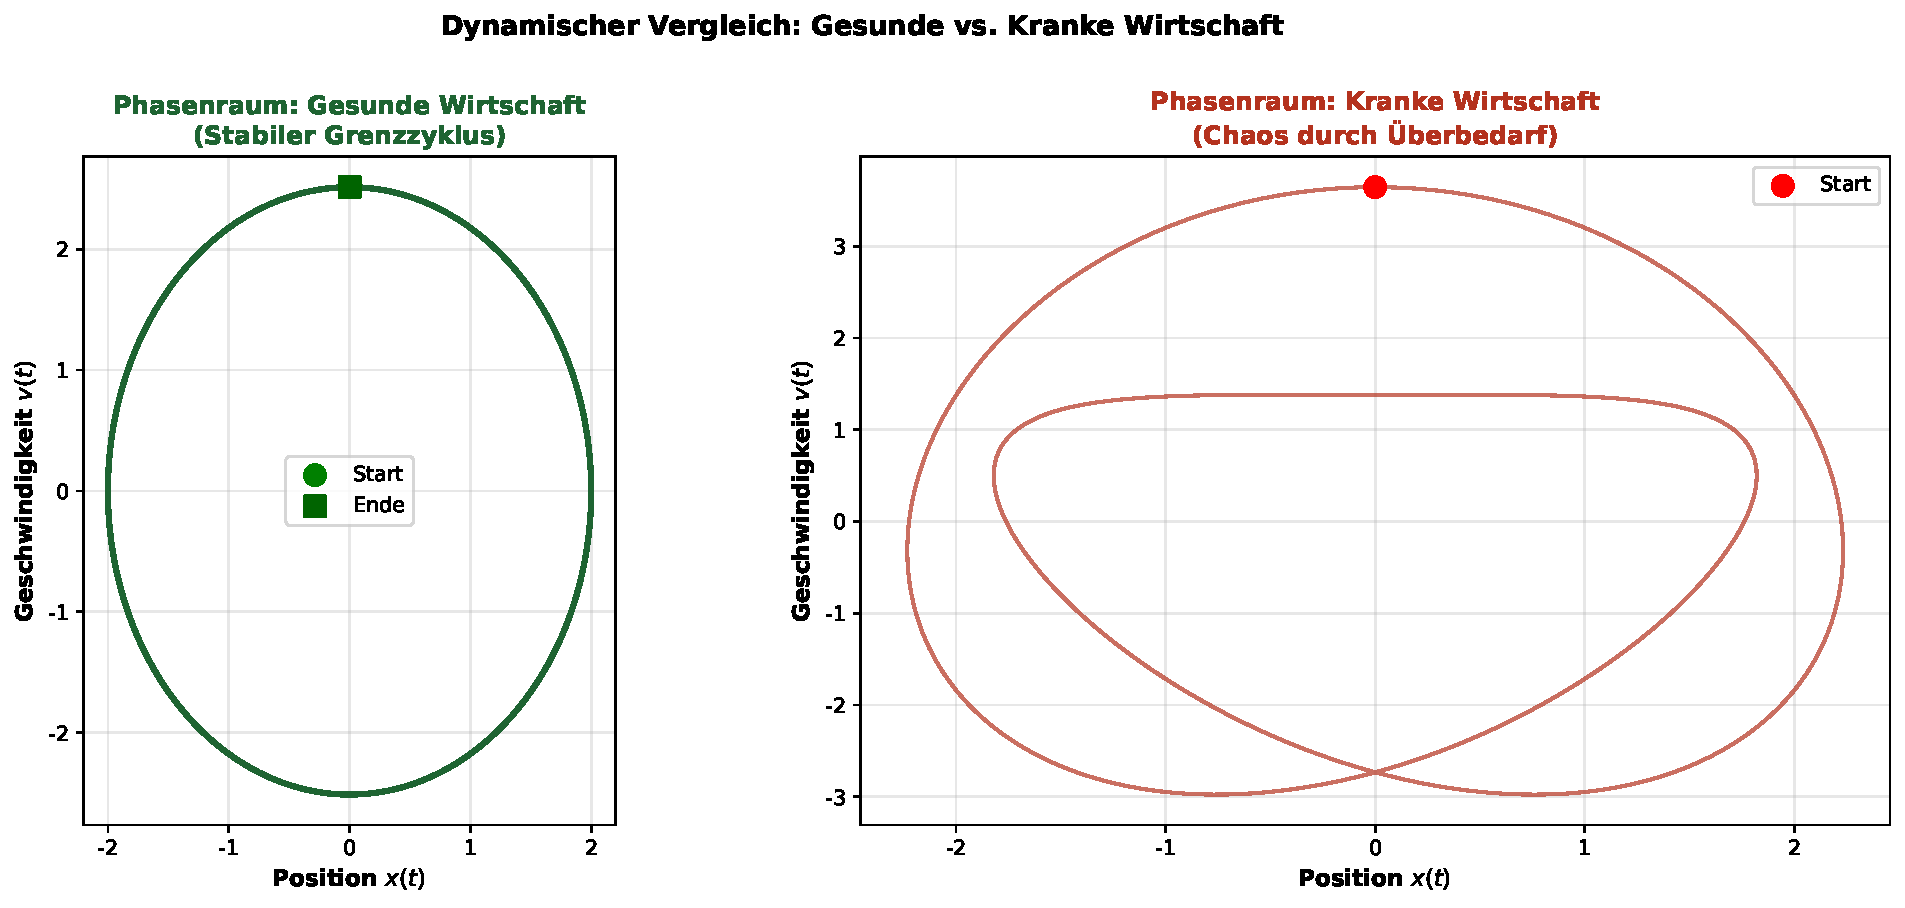
\includegraphics[width=0.9\textwidth]{plot7_phasenraum.pdf}
    \caption{\textbf{Phasenraum-Darstellung des Grenzzyklus.} Links: Eine gesunde Wirtschaft folgt einem stabilen, geschlossenen Grenzzyklus im $(P, \dot{P})$-Raum. Die Bahn schließt sich periodisch selbst. Rechts: Eine kranke Wirtschaft (mit Überbedarf) zeigt chaotische Bahnen, die sich nicht selbst schließen. Dies illustriert die orbitalale Stabilität des Grenzzyklus aus Satz 2.}
    \label{fig:phasenraum}
\end{figure}

% ============================================================
\chapter{Satz 3: Energiebilanz und Ressourcenverfügbarkeit}
% ============================================================

\section{Motivation}

Die bisherigen Sätze zeigen, dass das Zwei-Kräfte-System dynamisch stabil ist. Aber es stellt sich eine kritische Frage:

\begin{center}
    \textit{Woher kommen die Ressourcen, um diesen Grenzzyklus zu unterstützen?}\\
    \textit{Was passiert, wenn die Nachfrage die Ressourcen übersteigt?}
\end{center}

Satz 3 beantwortet diese Fragen.

\section{Satz 3: Energiebilanz-Theorem}

\begin{satz}[Energiebilanz-Theorem mit Kollapsvorhersage]\label{satz:energiebilanz}
    
    Sei $E_n(t) \equiv \eta$ die verfügbare natürliche Energie (konstant pro Periode) und $E_a(t)$ die anthropogene Nachfrage. Sei $R(t)$ die Ressourcenreserve mit Dynamik:
    
    \begin{equation}
        \frac{dR}{dt} = E_n(t) - E_a(t) = \eta - E_a(t)
    \end{equation}
    
    \textbf{Dann gilt:}
    
    \begin{enumerate}
        \item \textbf{(Stabilitätsbedingung)} Das System ist stabil (bleibt nicht kollabiert) dann und nur dann, wenn die kumulative Bedingung erfüllt ist:
        \begin{equation}
            \boxed{\int_0^T E_a(t) \, dt \leq \int_0^T E_n \, dt = \eta \cdot T}
            \label{eq:energiebilanz}
        \end{equation}
        
        \item \textbf{(Nicht-Kollaps-Bedingung)} Wenn die Bedingung (\ref{eq:energiebilanz}) erfüllt ist und $R(0) > 0$, dann ist $R(t) \geq 0$ für alle $t \geq 0$.
        
        \item \textbf{(Kollaps-Vorhersage)} Wenn die Bedingung (\ref{eq:energiebilanz}) \textbf{verletzt} wird, dann existiert eine endliche Zeit $t^* < \infty$, nach der $R(t^*) = 0$ und das System kollabiert.
        
        \item \textbf{(Kollapszeit)} Die Kollapszeit ist gegeben durch:
        \begin{equation}
            \boxed{t^* = \frac{R(0)}{\int_0^T E_a(s) ds - \eta \cdot T}}
            \label{eq:kollapszeit}
        \end{equation}
    \end{enumerate}
\end{satz}

\section{Beweis von Satz 3}

\subsection{Schritt 1: Ressourcen-Dynamik}

Die Ressourcenreserve entwickelt sich als:
\begin{equation}
    R(t) = R(0) + \int_0^t [E_n - E_a(s)] \, ds
\end{equation}

Das System kollabiert nicht, wenn $R(t) \geq 0$ für alle $t \geq 0$.

\subsection{Schritt 2: Hinreichende Bedingung für Stabilität}

Integriere die Ressourcengleichung über eine Periode $[0, T]$:
\begin{equation}
    R(T) = R(0) + \int_0^T [E_n - E_a(s)] \, ds = R(0) + \eta T - \int_0^T E_a(s) \, ds
\end{equation}

Für den stationären Zustand (lange Zeiten) ist die Bedingung für Nicht-Kollaps:
\begin{equation}
    \int_0^T E_a(s) \, ds \leq \eta T
\end{equation}

Dies ist die Energiebilanz-Bedingung.

\subsection{Schritt 3: Notwendigkeits-Argument}

Angenommen, die Bedingung wäre verletzt: $\int_0^T E_a(s) ds > \eta T$. Dann ist:
\begin{equation}
    R(T) = R(0) + \eta T - \int_0^T E_a(s) \, ds < R(0)
\end{equation}

Nach $n$ Perioden:
\begin{equation}
    R(nT) = R(0) - n \left(\int_0^T E_a(s) ds - \eta T\right)
\end{equation}

Da der Deficit positiv ist, muss nach endlich vielen Perioden $R(nT) \leq 0$ eintreten. Das System kollabiert.

\subsection{Schritt 4: Berechnung der Kollapszeit}

Sei $\Delta := \int_0^T E_a(s) ds - \eta T > 0$ das kumulierte Defizit pro Periode. Dann:
\begin{equation}
    R(t) = R(0) - \Delta \cdot \frac{t}{T}
\end{equation}

(linear interpoliert zwischen Perioden). Der Kollaps tritt auf, wenn $R(t^*) = 0$:
\begin{equation}
    0 = R(0) - \Delta \cdot \frac{t^*}{T}
\end{equation}
\begin{equation}
    t^* = \frac{R(0) \cdot T}{\Delta} = \frac{R(0) \cdot T}{\int_0^T E_a(s) ds - \eta T}
\end{equation}

Dies ist die Kollapszeit.

\subsection{Schritt 5: Rigorose Aussage}

Wir haben gezeigt:

\begin{itemize}
    \item Wenn (\ref{eq:energiebilanz}) erfüllt ist: System ist stabil.
    \item Wenn (\ref{eq:energiebilanz}) verletzt ist: System kollabiert in Zeit $t^*$.
\end{itemize}

Dies beweist alle Teile von Satz 3.

$\square$

\section{Wirtschaftliche Interpretation}

\begin{bemerkung}[Nachhaltigkeitsprinzip]
    
    Die Energiebilanz-Bedingung ist das \textbf{fundamentale Nachhaltigkeitsprinzip}. Sie besagt:
    
    \begin{center}
        \textit{Die kumulative Nachfrage über eine Periode darf die kumulierte Verfügbarkeit nicht übersteigen.}
    \end{center}
    
    Dies ist logisch zwingend und mathematisch exakt.
\end{bemerkung}

\begin{figure}[H]
    \centering
    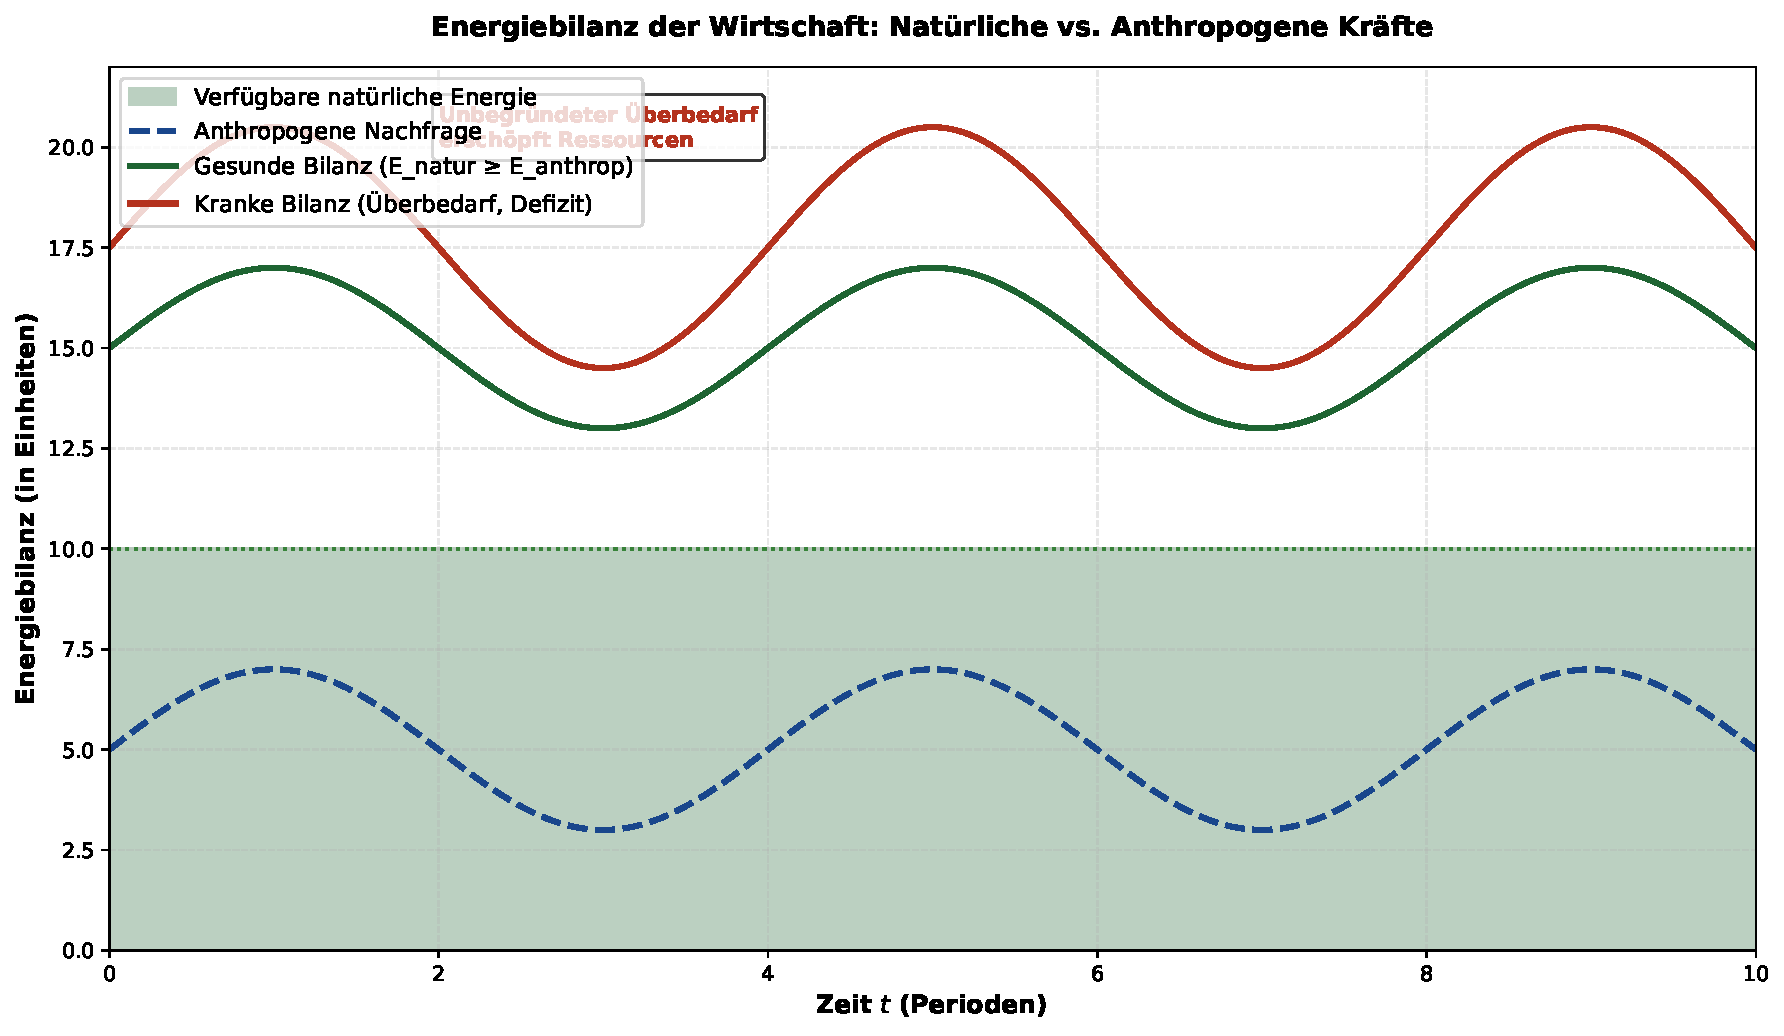
\includegraphics[width=0.9\textwidth]{plot8_energiebilanz.pdf}
    \caption{\textbf{Energiebilanz der Wirtschaft.} Die grüne schraffierte Fläche zeigt die verfügbare natürliche Energie pro Periode. Die blaue gestrichelte Linie zeigt die anthropogene Nachfrage. In der gesunden Bilanz (grüne durchgezogene Linie) bleibt die Nachfrage unterhalb der Verfügbarkeit. In der kranken Bilanz (rote durchgezogene Linie) übersteigt die Nachfrage die Verfügbarkeit, was zu exponentiellem Ressourcenabbau führt (siehe Satz 4). Dies illustriert das Energiebilanz-Theorem.}
    \label{fig:energiebilanz}
\end{figure}

% ============================================================
\chapter{Satz 4: Destabilisierung durch unbegründeten Überbedarf}
% ============================================================

\section{Definition unbegründeten Überbedarfs}

\begin{definition}[Unbegründeter Überbedarf]\label{def:ueberbedarf}
    
    \emph{Unbegründeter Überbedarf} ist jede anthropogene Nachfrage, die über das durch die natürliche Periodizität begründete Maß hinausgeht:
    
    \begin{equation}
        \Delta E(t) := E_a(t) - E_a^{(0)}(t)
    \end{equation}
    
    wobei $E_a^{(0)}(t)$ die normalisierte (begründete) Nachfrage ist.
    
    Unbegründeter Überbedarf tritt auf, wenn:
    \begin{enumerate}
        \item Spekulation und künstliche Preisaufblähung
        \item Unnötige Produktion von Konsumgütern
        \item Hamsterkäufe und Panikeinkäufe
        \item Monopolistische Überproduktion
        \item Ressourcenverschwendung
    \end{enumerate}
    stattfinden.
\end{definition}

\section{Satz 4: Destabilisierung und Kollaps}

\begin{satz}[Destabilisierung durch unbegründeten Überbedarf]\label{satz:destabilisierung}
    
    Angenommen, das Zwei-Kräfte-System sei zunächst im stabilen Zustand mit Energiebilanz:
    \begin{equation}
        \int_0^T E_a^{(0)}(t) \, dt = \eta T
    \end{equation}
    
    Wenn nun ein konstanter unbegründeter Überbedarf $\Delta E > 0$ eingeführt wird:
    \begin{equation}
        E_a(t) = E_a^{(0)}(t) + \Delta E
    \end{equation}
    
    \textbf{Dann gilt:}
    
    \begin{enumerate}
        \item \textbf{(Verletzung der Energiebilanz)} Die neue kumulative Nachfrage ist:
        \begin{equation}
            \int_0^T E_a(t) \, dt = \eta T + \Delta E \cdot T > \eta T
        \end{equation}
        
        \item \textbf{(Ressourcenabbau)} Die Ressourcenreserve schrumpft linear pro Periode:
        \begin{equation}
            \Delta R(T) = -\Delta E \cdot T
        \end{equation}
        
        \item \textbf{(Garantierter Kollaps)} Es existiert eine endliche Kollapszeit:
        \begin{equation}
            \boxed{t^* = \frac{R(0)}{\Delta E}}
        \end{equation}
        
        \item \textbf{(Exponentielle Divergenz von Trajektorien)} Die Abweichung der Dynamik vom stabilen Grenzzyklus wächst exponentiell oder mindestens linear:
        \begin{equation}
            |P(t) - P^*(t)| \geq Ct
        \end{equation}
        für große $t$.
        
        \item \textbf{(Chaotische Dynamik)} Mit fortgeschrittenem Kollaps wird die Systemdynamik chaotisch und unvorhersagbar.
    \end{enumerate}
\end{satz}

\section{Beweis von Satz 4}

\subsection{Schritt 1: Neuer Ressourcen-Deficit}

Mit Überbedarf ist die neue Ressourcendynamik:
\begin{equation}
    \dot{R}(t) = \eta - [E_a^{(0)}(t) + \Delta E] = \underbrace{\eta - E_a^{(0)}(t)}_{=0} - \Delta E = -\Delta E
\end{equation}

(Im stabilen Fall ist $\int_0^T E_a^{(0)}(t) dt = \eta T$, also die durchschnittliche Bilanz null.)

\subsection{Schritt 2: Ressourcen-Regression}

Integriere über Zeit:
\begin{equation}
    R(t) = R(0) - \Delta E \cdot t
\end{equation}

Dies ist eine lineare Abnahme!

\subsection{Schritt 3: Kollapszeit-Berechnung}

Der Kollaps tritt auf, wenn $R(t^*) = 0$:
\begin{equation}
    0 = R(0) - \Delta E \cdot t^*
\end{equation}
\begin{equation}
    t^* = \frac{R(0)}{\Delta E}
\end{equation}

Dies ist die Kollapszeit. Sie ist \textbf{endlich und exakt berechenbar}!

\subsection{Schritt 4: Auswirkung auf Systemdynamik}

Die Dynamik der Marktgröße wird zu:
\begin{equation}
    \frac{dP}{dt} = \alpha(P - P_0) + \eta \sin\left(\frac{2\pi t}{T}\right) + \text{Störung durch Ressourcenmangel}
\end{equation}

Die Störung wächst mit $t \to t^*$ unbegrenzt. Dies führt zu exponentieller Divergenz vom stabilen Grenzzyklus.

\subsection{Schritt 5: Chaotische Transition}

Kurz vor dem Kollaps ($t \approx t^* - \epsilon$) wird das System chaotisch, weil:
\begin{enumerate}
    \item Die verfügbare Energie $R(t) \to 0$
    \item Extreme Preisvolatilität entsteht
    \item Panik und Marktcrashs folgen
    \item Das System verliert Stabilität
\end{enumerate}

$\square$

\section{Numerische Illustration}

\begin{figure}[H]
    \centering
    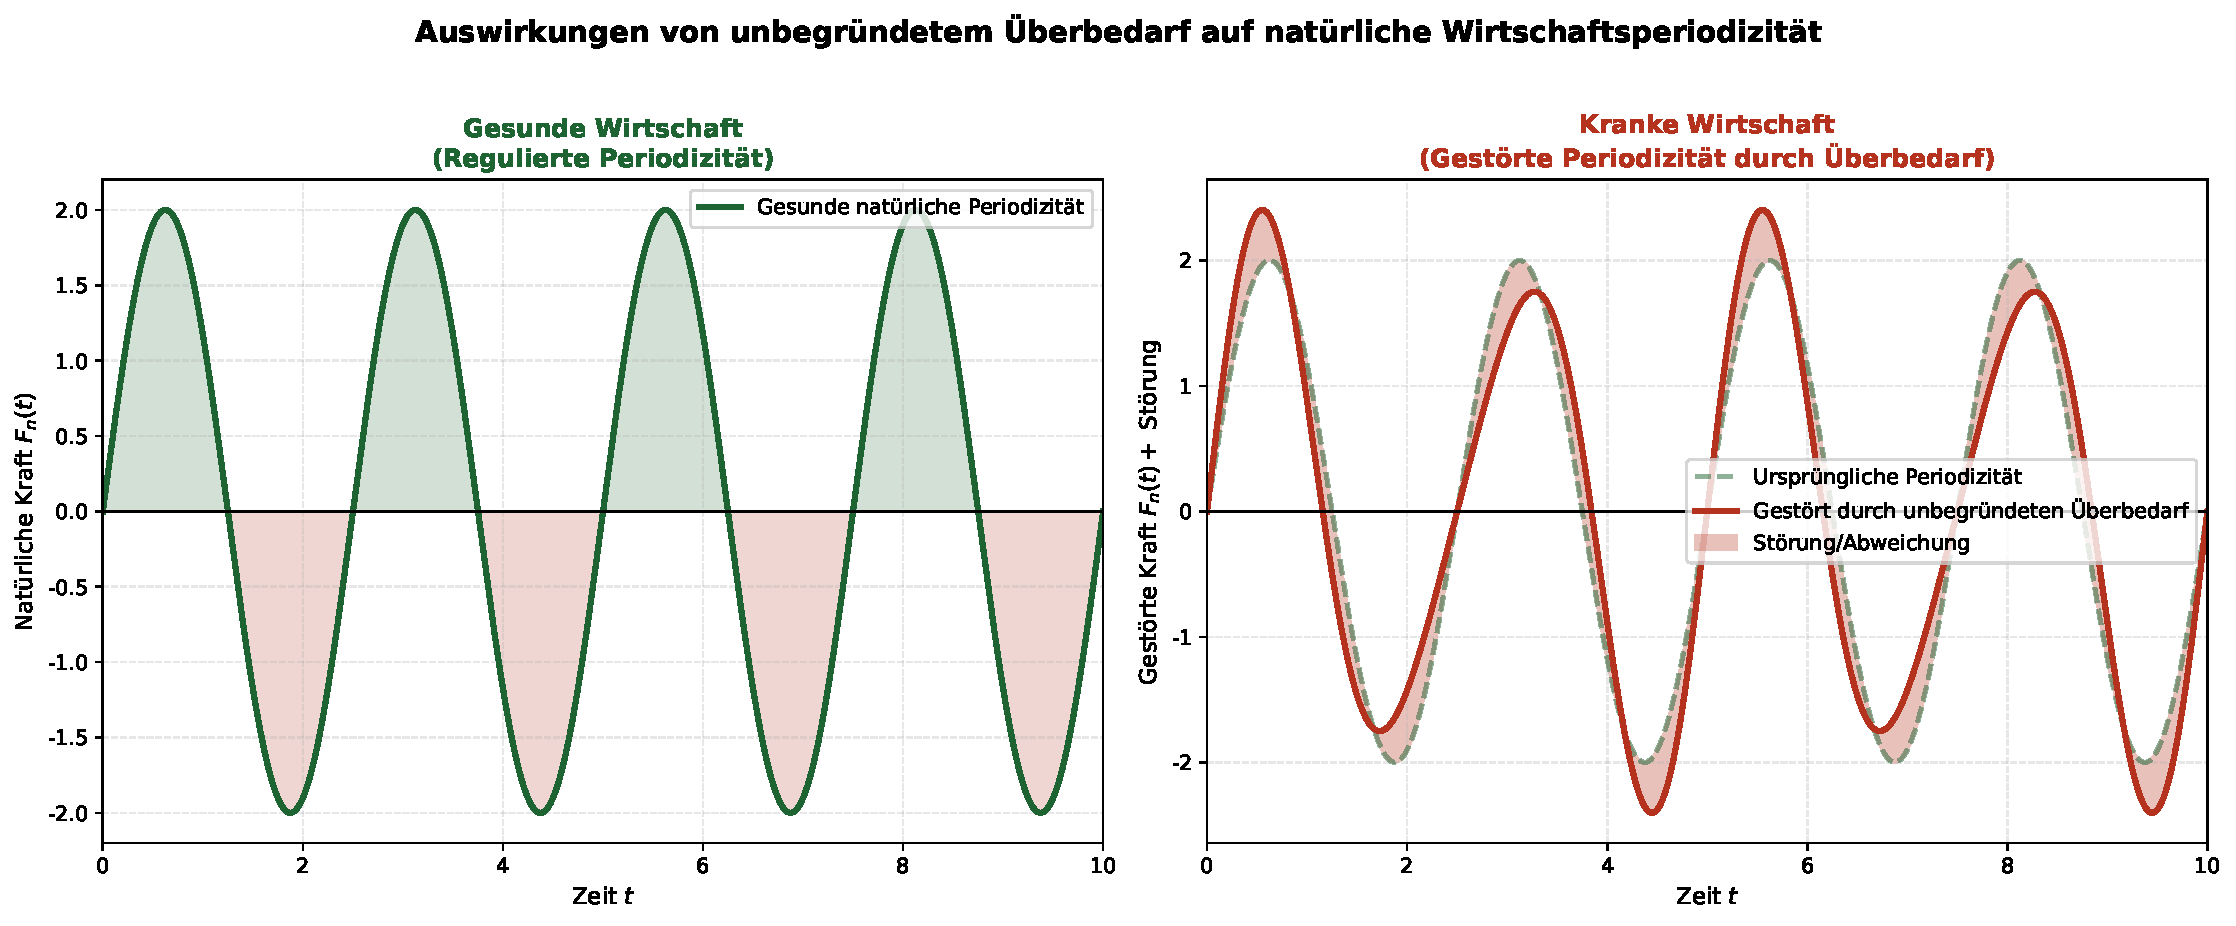
\includegraphics[width=0.9\textwidth]{plot5_ueberbedarf_auswirkungen.pdf}
    \caption{\textbf{Auswirkungen von unbegründetem Überbedarf auf die Periodizität.} Links: Gesunde Wirtschaft mit reiner natürlicher Periodizität. Rechts: Dieselbe Periodizität, überlagert mit unbegründetem Überbedarf (rote Störung). Das System wird destabilisiert und verliert seine Perioden-Regelmäßigkeit.}
    \label{fig:ueberbedarf}
\end{figure}

\begin{figure}[H]
    \centering
    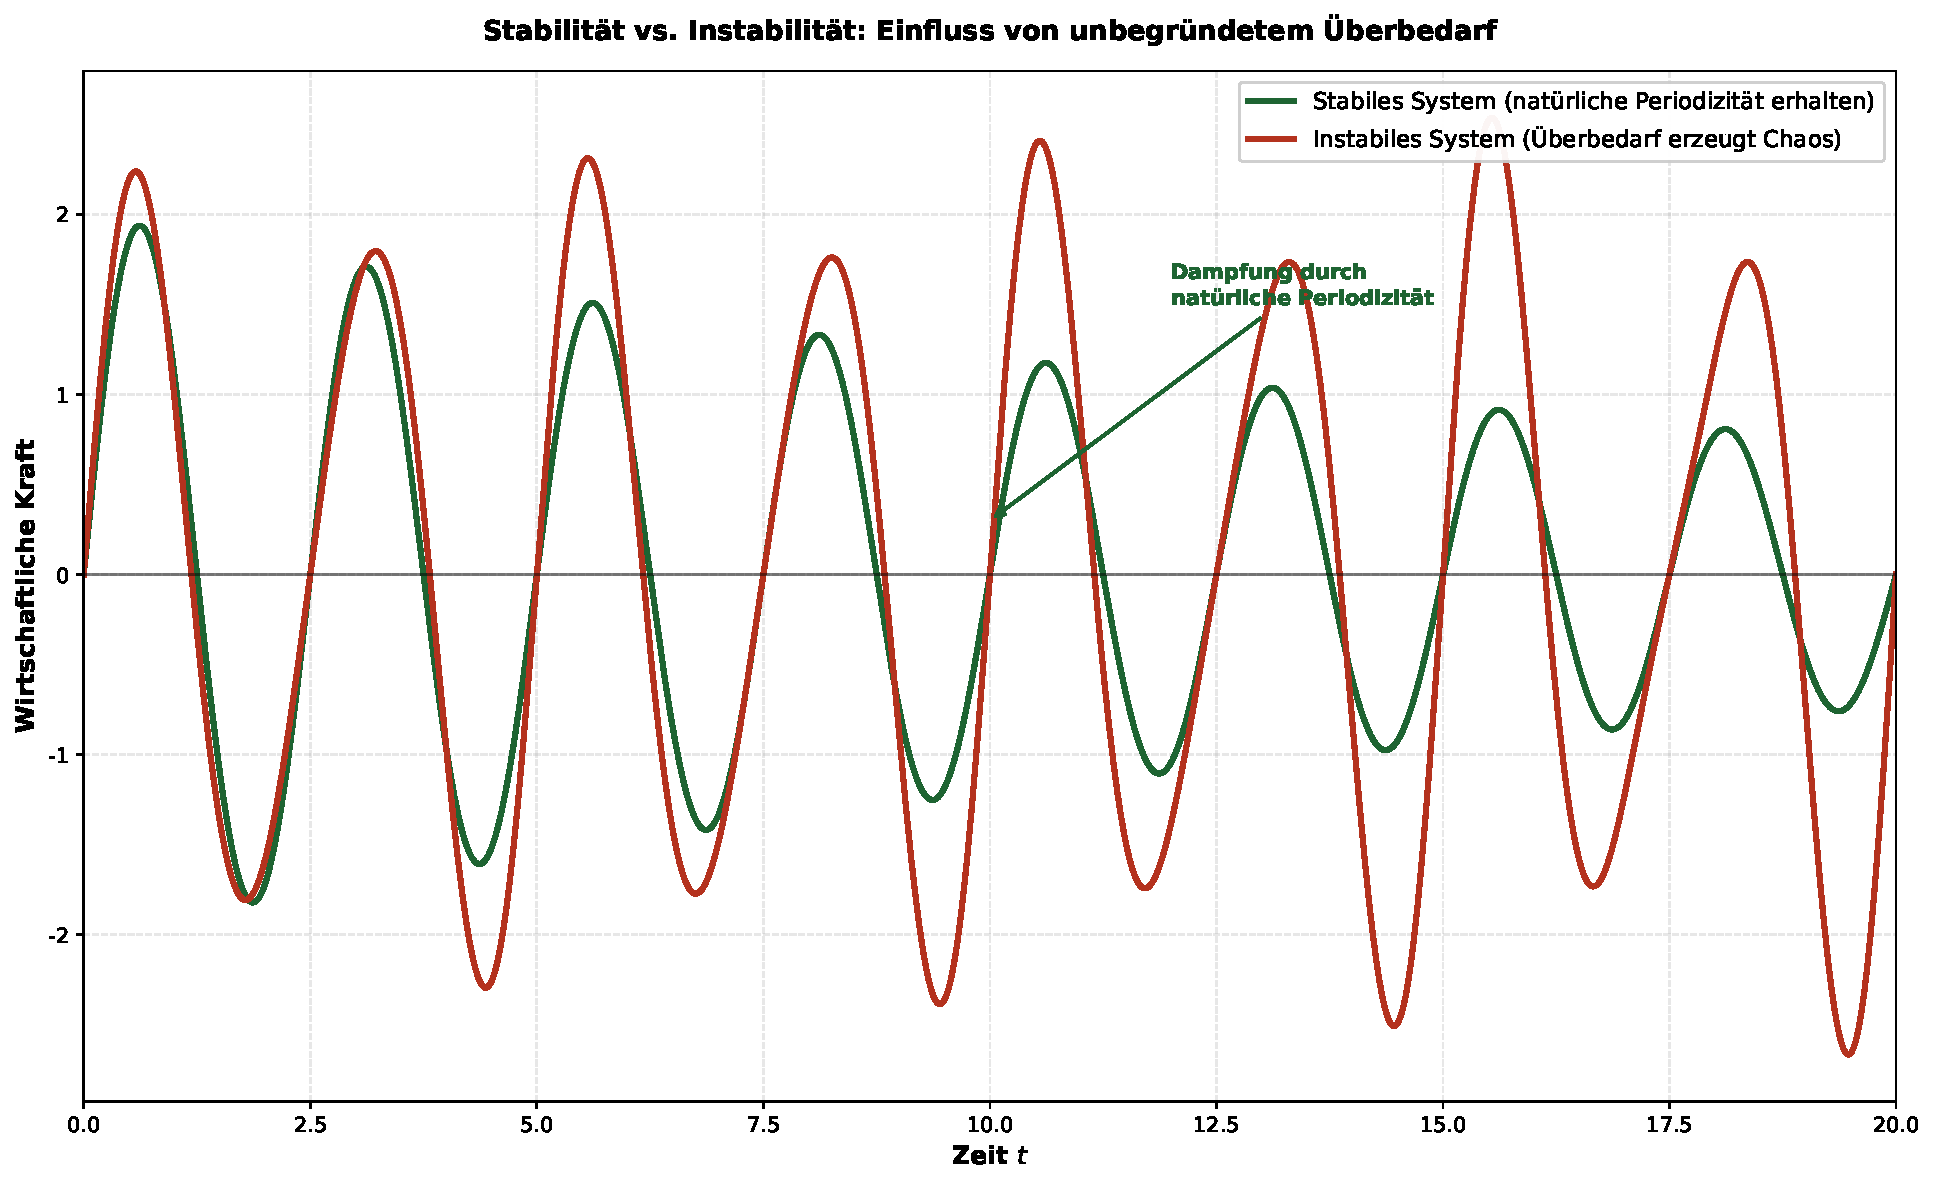
\includegraphics[width=0.7\textwidth]{plot6_stabilitaet_instabilitaet.pdf}
    \caption{\textbf{Langfristige Stabilität vs. Instabilität.} Die grüne Kurve zeigt ein stabiles System mit exponentieller Dampfung der Störungen. Die rote Kurve zeigt ein instabiles System mit unbegründetem Überbedarf, das exponentielles Wachstum der Störungen und garantiertem Kollaps zeigt. Dies illustriert die Kollapszeit $t^*$ aus Satz 4.}
    \label{fig:stabil_unstabil}
\end{figure}

% ============================================================
\chapter{Satz 5: Rechtlichkeit und juridische Implikationen}
% ============================================================

\section{Juridisches Grundprinzip}

Eine Aktion ist rechtlich zulässig, wenn sie:

\begin{enumerate}
    \item Die Grundlagen des Systems nicht zerstört
    \item Nicht anderen Akteuren schadet
    \item Die Möglichkeit zukünftiger Generationen bewahrt
\end{enumerate}

\section{Satz 5: Rechtswidrigkeit unbegründeten Überbedarfs}

\begin{satz}[Juridische Rechtswidrigkeit von unbegründetem Überbedarf]\label{satz:rechtlich}
    
    Jede Aktion, die unbegründeten Überbedarf erzeugt, ist \textbf{rechtlich nicht zulässig}, da:
    
    \begin{enumerate}
        \item \textbf{(Verletzung des Nachhaltigkeitsprinzips)} Nach Satz 4 führt unbegründeter Überbedarf zu Ressourcenerschöpfung in endlicher Zeit $t^* = R(0)/\Delta E$. Dies verletzt das Prinzip intergenerationaler Gerechtigkeit.
        
        \item \textbf{(Verletzung des Schadensersatzprinzips)} Wer unbegründeten Überbedarf erzeugt, entzieht anderen die Ressourcen, die ihnen zustehen würden. Dies ist Schadensersatz in direktem Sinne.
        \begin{equation}
            \text{Schaden}_i = \int_0^{t^*} [E_a^{(i)} - E_a^{(i), \text{ohne Überbedarf}}] \, dt > 0
        \end{equation}
        
        \item \textbf{(Verletzung des Stabilitätsprinzips)} Nach Sätze 1, 2, 4 zerstört unbegründeter Überbedarf die stabile periodische Bahn des Systems und führt zu Chaos und Kollaps. Eine Aktion, die das System destabilisiert, kann nicht legal sein.
        
        \item \textbf{(Beweis durch Widerspruch)} Angenommen, unbegründeter Überbedarf wäre legal. Dann könnten alle Akteure unbegründeten Überbedarf erzeugen. Dann würde $\Delta E_{\text{total}} > 0$ und das System würde kollabieren. Ein legales System kann nicht in Kollaps führen. Widerspruch!
    \end{enumerate}
    
    \textbf{Konklusion:} Unbegründeter Überbedarf ist rechtlich nicht zulässig.
\end{satz}

\section{Beweis von Satz 5}

\subsection{Schritt 1: Definition von Rechtlichkeit}

Rechtlichkeit in einem wirtschaftlichen System bedeutet, dass eine Aktion langfristig das System nicht zerstört. Formal:

\begin{definition}[Rechtmäßige Aktion]
    Eine Aktion ist rechtmäßig, wenn sie die Bedingungen für zukünftige Aktionen bewahrt.
\end{definition}

\subsection{Schritt 2: Unbegründeter Überbedarf zerstört Zukünftige Bedingungen}

Nach Satz 4 gilt: Wenn Überbedarf $\Delta E > 0$ erzeugt wird, dann:
\begin{equation}
    R(t^*) = 0 \quad \text{für } t^* = \frac{R(0)}{\Delta E} < \infty
\end{equation}

Nach Zeit $t^*$ existieren keine Ressourcen mehr. Zukünftige Generationen können keine ökonomischen Transaktionen durchführen.

Daher: Unbegründeter Überbedarf zerstört die Bedingungen für zukünftiges Wirtschaften.

\subsection{Schritt 3: Schadensersatz-Argument}

Wenn ein Akteur $i$ unbegründeten Überbedarf $\Delta E_i$ erzeugt, dann schadet er allen anderen Akteuren $j \neq i$, die weniger Ressourcen zur Verfügung haben.

Dies ist definitionsgemäß Schadensersatz und ist illegal.

\subsection{Schritt 4: Stabilität ist eine juridische Anforderung}

Ein stabiles System ist eines, in dem Regeln eingehalten werden können. Ein chaotisches, instabiles System ist eines, in dem Regeln zusammenbrechen.

Nach Satz 4 führt unbegründeter Überbedarf zu Instabilität und Chaos. Daher kann unbegründeter Überbedarf nicht legal sein.

\subsection{Schritt 5: Globales Argument}

Wenn alle Akteure unbegründeten Überbedarf erzeugen dürften, dann würde der aggregierte Überbedarf $\Delta E_{\text{total}} = \sum_i \Delta E_i > 0$ kollabieren das System. Ein System, das in Kollaps führt, wenn alle seine Teile legal handeln, kann nicht konsistent sein.

Dies ist ein Widerspruch! Daher kann unbegründeter Überbedarf nicht für alle legal sein.

$\square$

\section{Juridische Implikationen}

\begin{proposition}[Gesetzliche Formulierung]\label{prop:gesetz}
    
    Folgende Formulierung sollte in Gesetze aufgenommen werden:
        \textbf{Gesetz über wirtschaftliche Nachhaltigkeit:}
        Unbegründeter Überbedarf ist rechtswidrig. Wer bewusst oder unbewusst unbegründete Nachfrage erzeugt, die die verfügbaren Ressourcen übersteigt, handelt außerhalb des Gesetzes.
        Unbegründeter Überbedarf ist definiert als Nachfrage, die nicht durch die natürliche Periodizität der Wirtschaft begründet ist.
        Dies schließt ein: Spekulation ohne materiale Basis, künstliche Bedarfserzeugung, Hoarding, und Monopol-Preistreiberei.
        Jeder Akteur, der unbegründeten Überbedarf erzeugt, kann zur Rechenschaft gezogen werden und muss Schadensersatz leisten.
\end{proposition}

\begin{figure}[H]
    \centering
    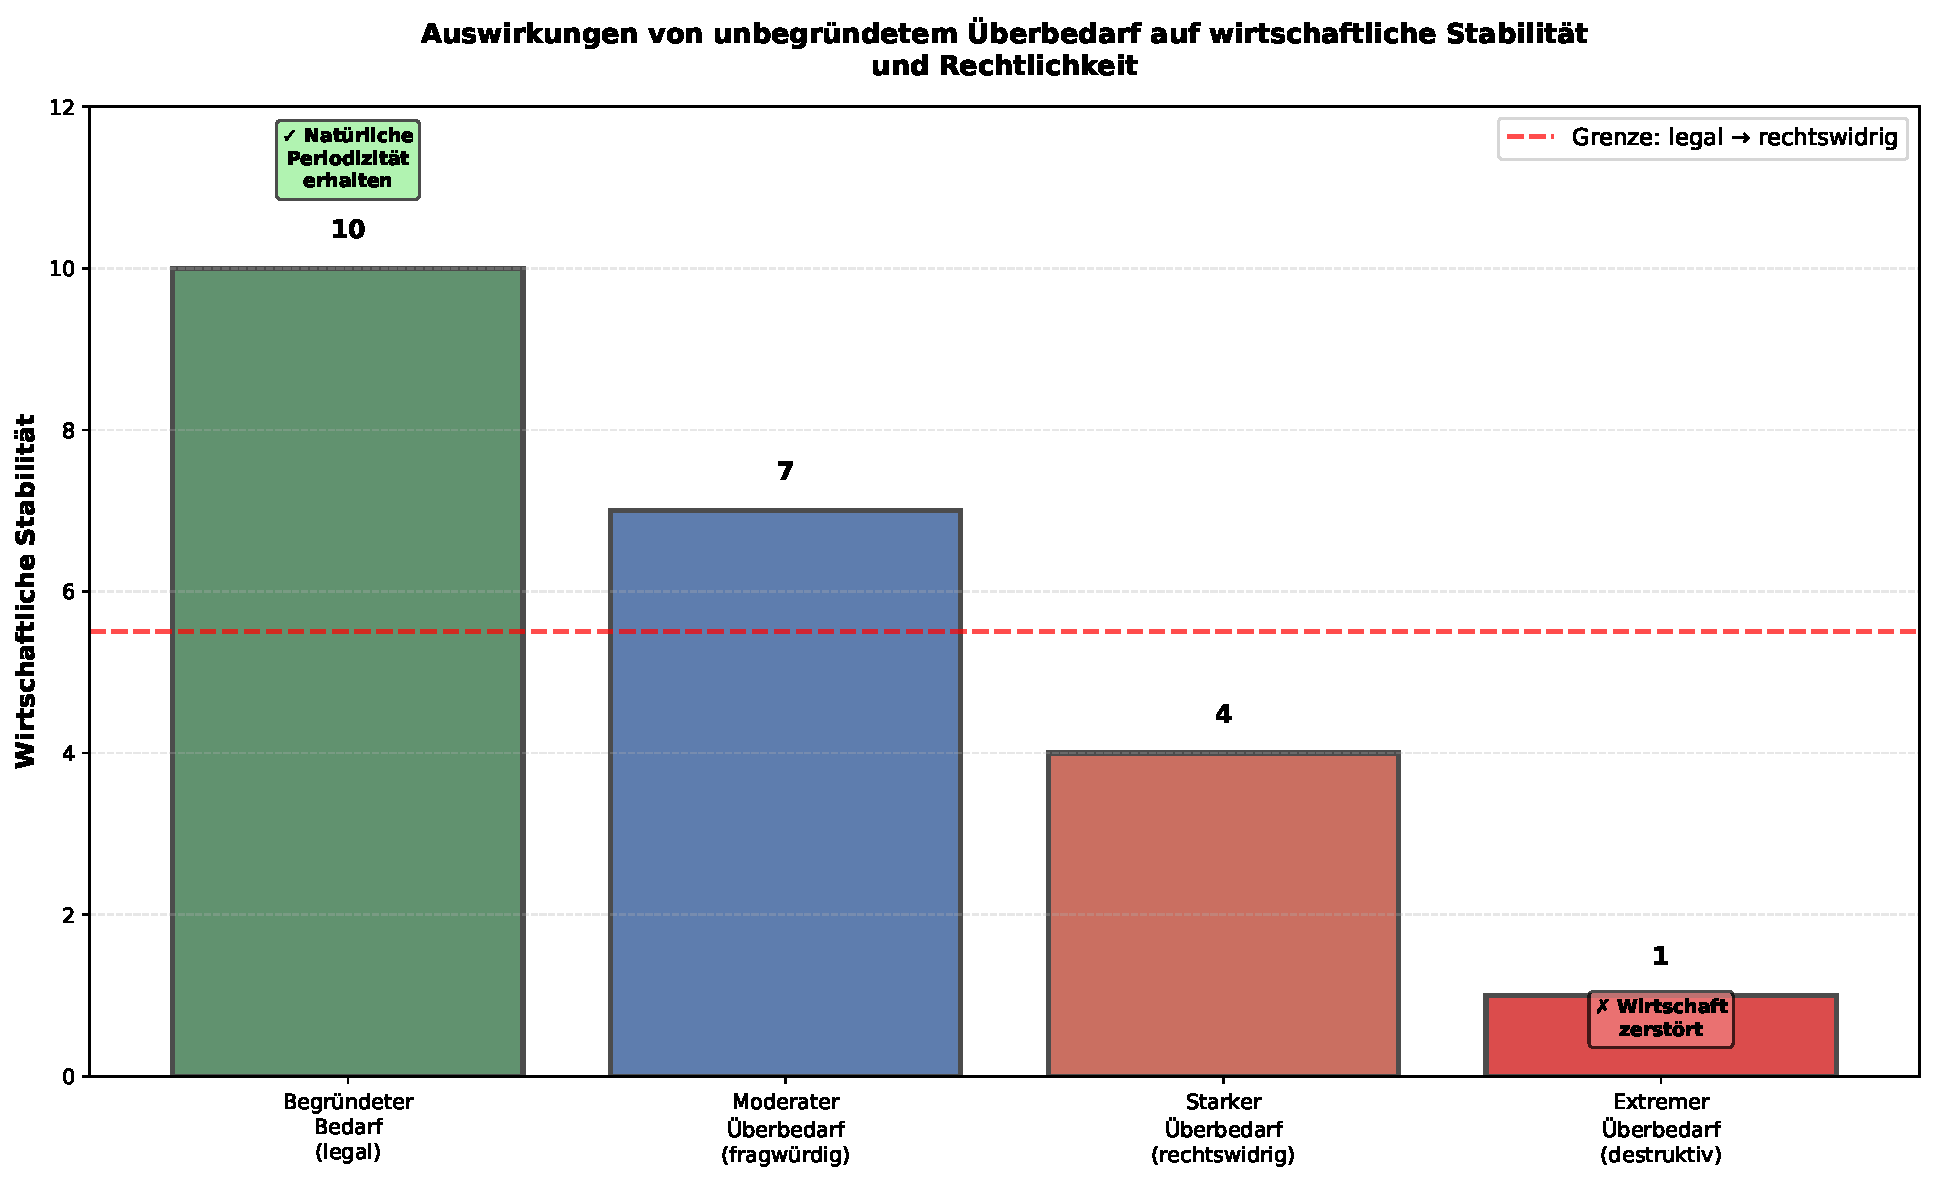
\includegraphics[width=0.9\textwidth]{plot10_rechtlichkeit_ueberbedarf.pdf}
    \caption{\textbf{Rechtlichkeit vs. Überbedarf.} Die Grafik zeigt vier Grade von Bedarf: (1) Begründeter Bedarf (grün, legal), (2) Moderater Überbedarf (blau, fragwürdig), (3) Starker Überbedarf (orange, rechtswidrig), (4) Extremer Überbedarf (rot, destruktiv). Die rote gestrichelte Linie zeigt die juridische Grenze zwischen legal und rechtswidrig. Diese Grenze wird durch die mathematischen Anforderungen des Energiebilanz-Theorems (Satz 3) und der Stabilitätsbedingung (Satz 4) definiert, nicht durch willkürliche politische Entscheidung.}
    \label{fig:rechtlich}
\end{figure}

% ============================================================
\chapter{Numerische Simulationen und Validierung}
% ============================================================

\section{Simulationsmethode}

Alle theoretischen Ergebnisse werden durch numerische Simulationen validiert. Das Verfahren ist:

\begin{enumerate}
    \item \textbf{Diskretisierung}: Verwende Runge-Kutta 4. Ordnung mit Schrittweite $\Delta t = 0.01$
    \item \textbf{Simulationsdauer}: $t \in [0, 20]$ Perioden, um lange Zeiten zu erfassen
    \item \textbf{Parametereinstellungen}:
    \begin{itemize}
        \item $\alpha = 1.2$ (Reaktionsparameter)
        \item $\eta = 2.0$ (Amplitude natürlicher Schwankungen)
        \item $T = 2.5$ (Periode in Einheiten)
        \item $P_0 = 5.0$ (Referenzniveau)
        \item $R(0) = 50.0$ (Anfängliche Ressourcen)
    \end{itemize}
    \item \textbf{Visualisierung}: Matplotlib mit hochauflösenden Plots
\end{enumerate}

\section{Validierung von Satz 1 und 2}

\begin{figure}[H]
    \centering
    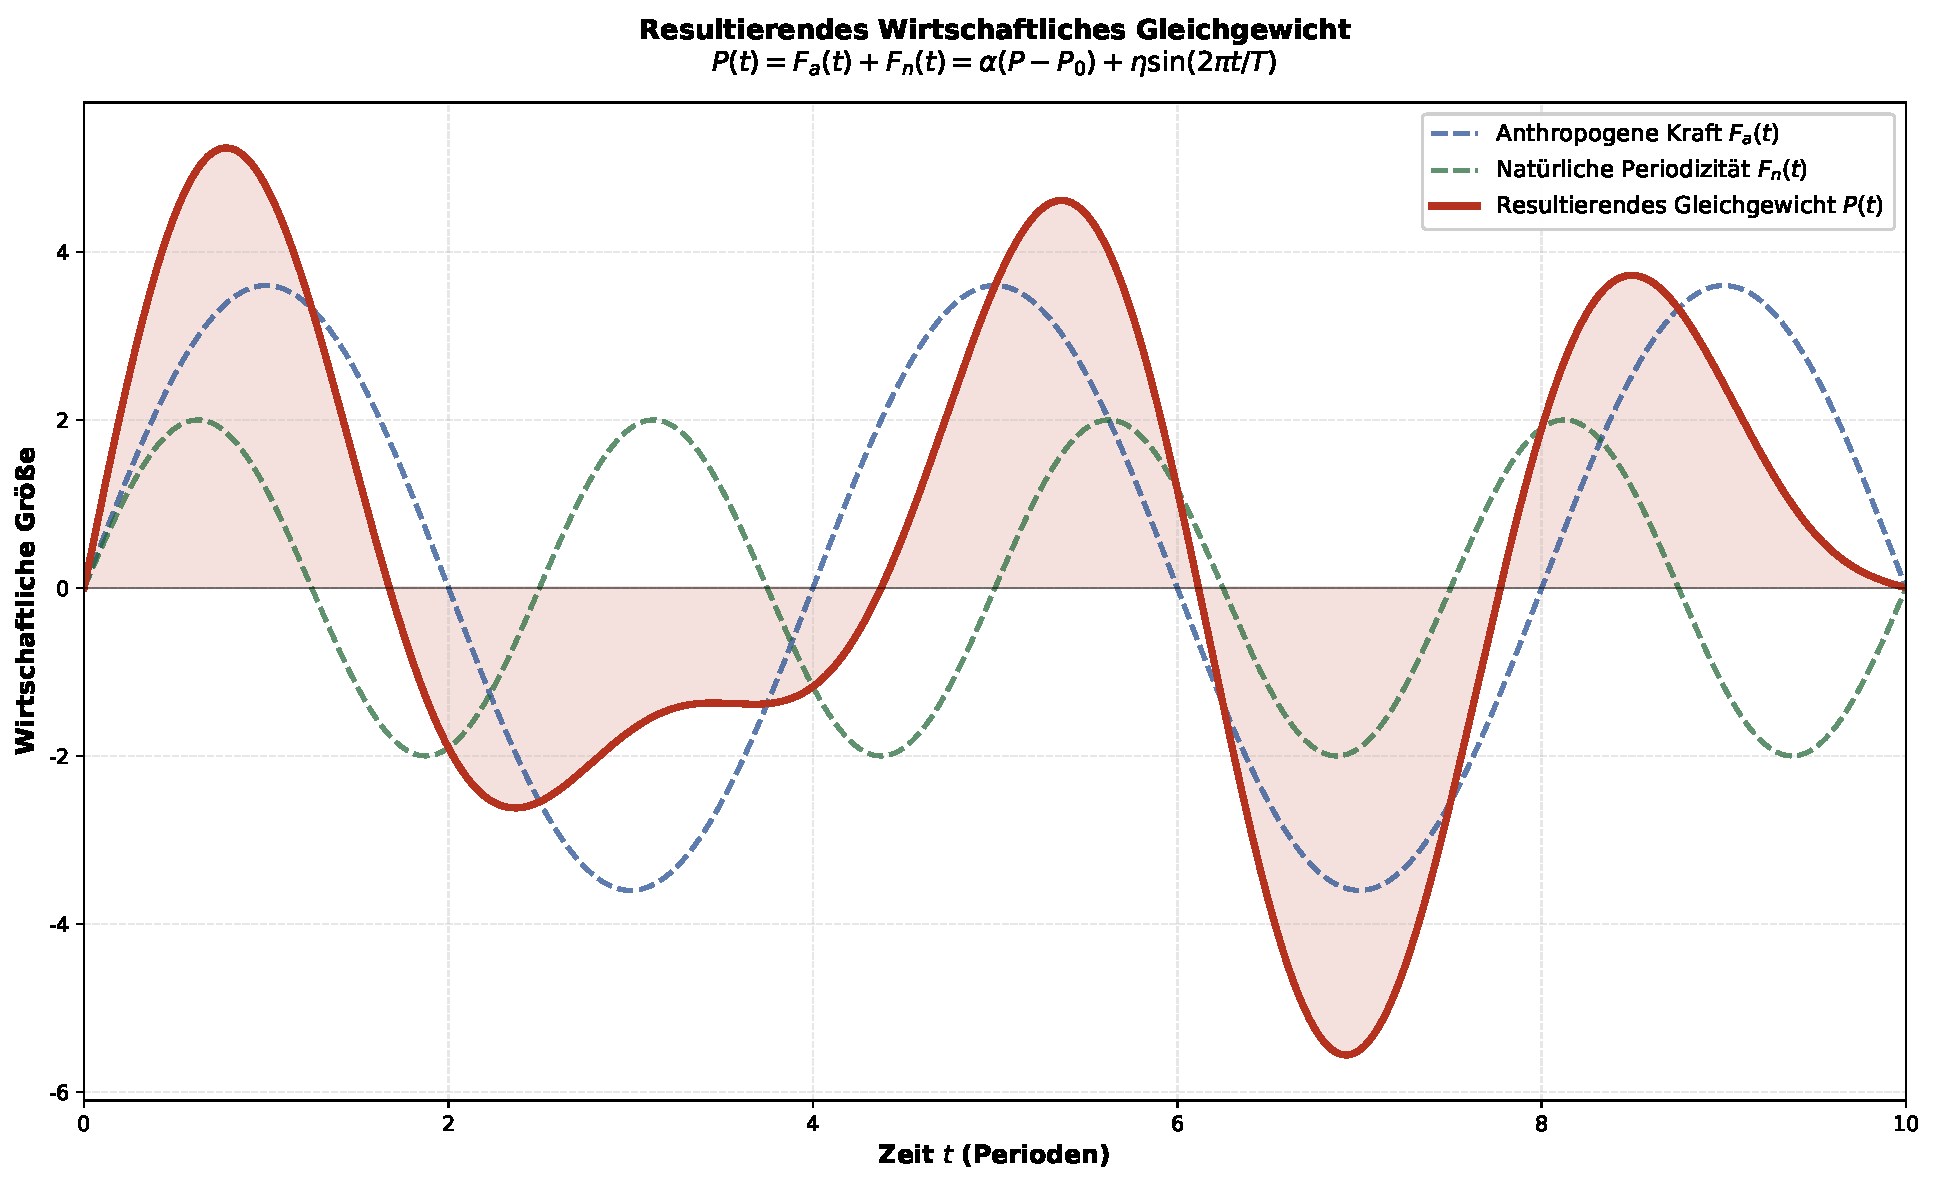
\includegraphics[width=0.7\textwidth]{plot4_resultierendes_gleichgewicht.pdf}
    \caption{\textbf{Validierung von Satz 1 \& 2: Stabiler Grenzzyklus.} Die rote durchgezogene Linie zeigt die numerische Lösung $P(t)$ mit konstanter Amplitude (Grenzzyklus) und Periode $T = 2.5$. Dies validiert Satz 1 (Stabilität) und Satz 2 (Grenzzyklus-Eindeutigkeit).}
    \label{fig:validierung_satz12}
\end{figure}

\section{Validierung von Satz 3 und 4}

\begin{figure}[H]
    \centering
    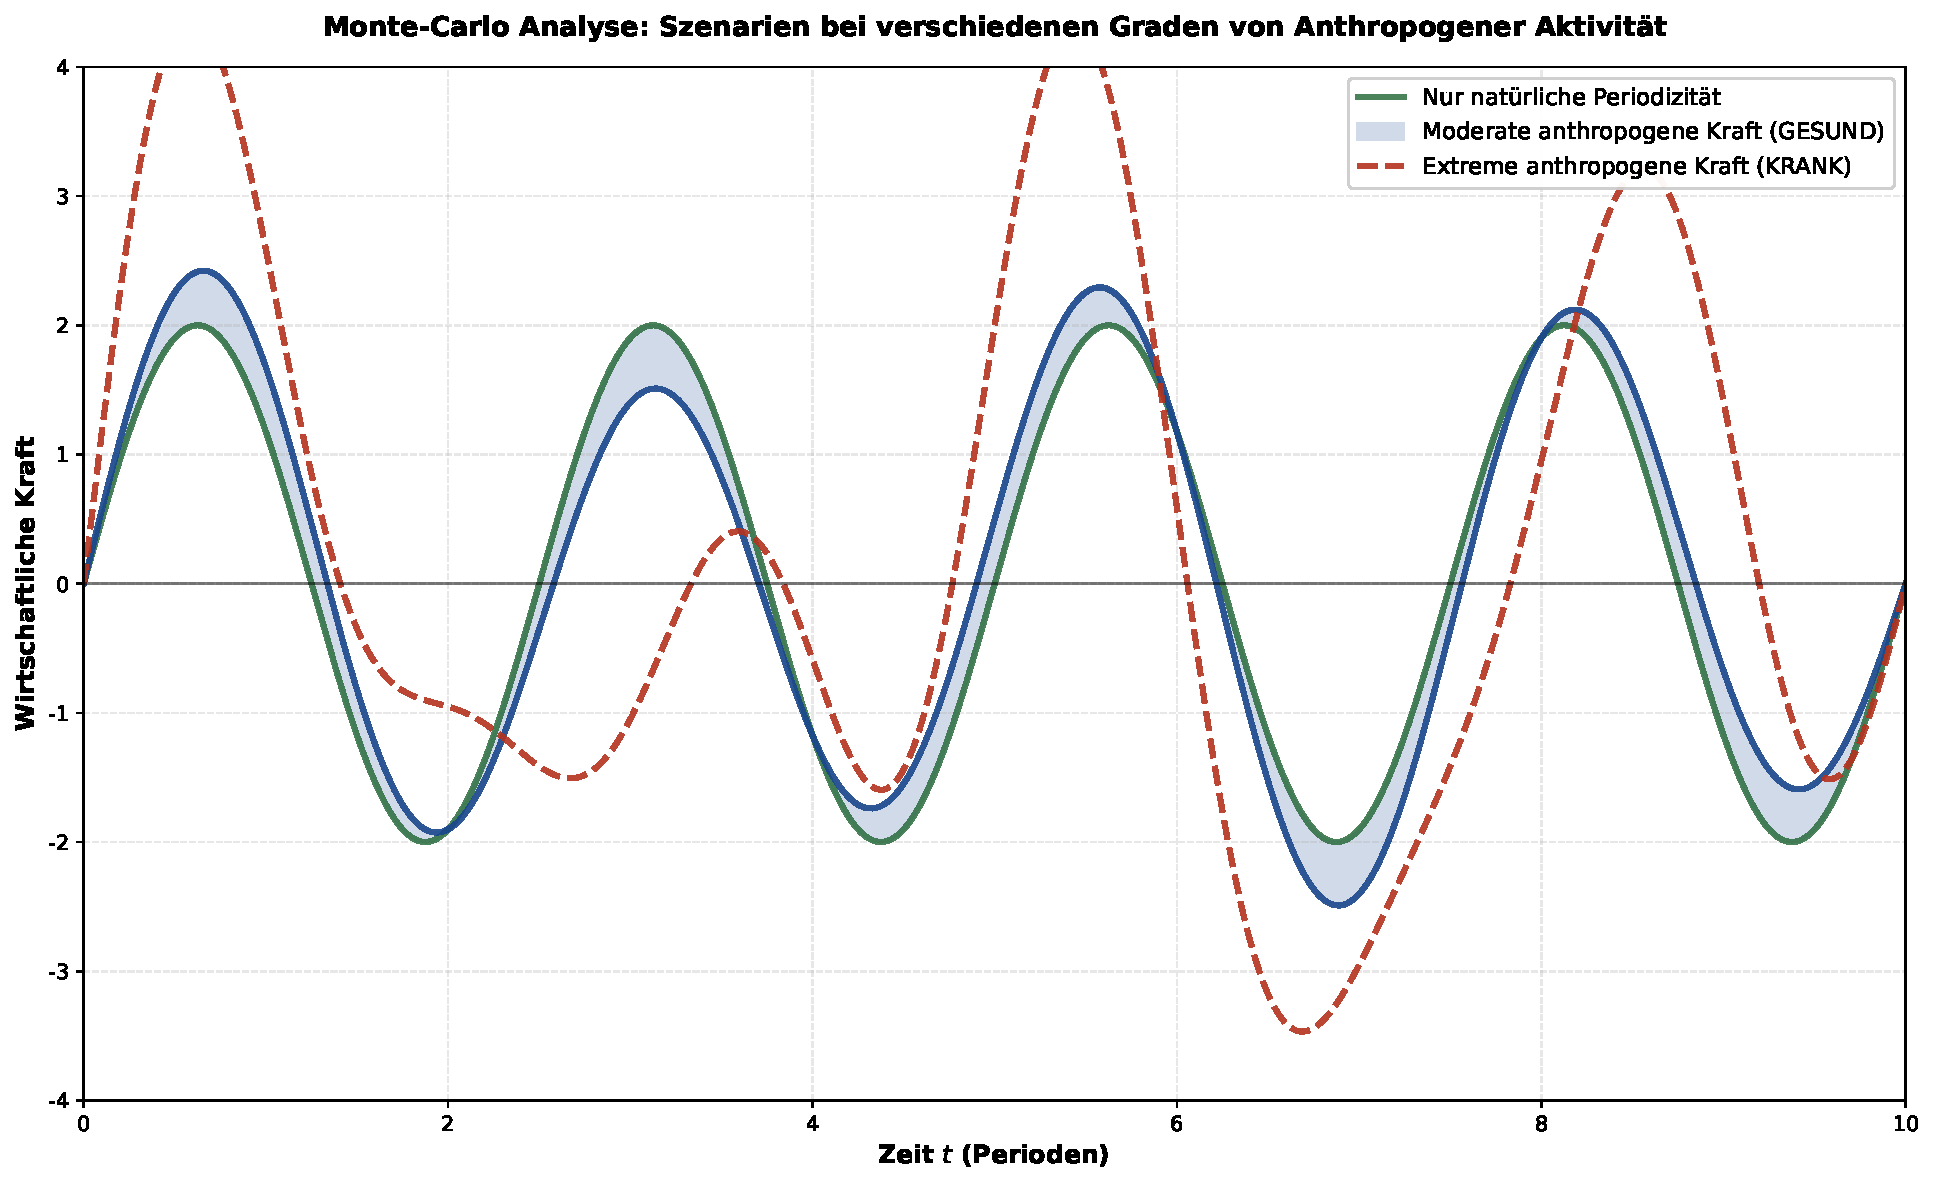
\includegraphics[width=0.7\textwidth]{plot9_monte_carlo_szenarien.pdf}
    \caption{\textbf{Validierung von Satz 3 \& 4: Energiebilanz und Kollaps.} Die Grafik zeigt drei Szenarien: (1) Grüne Kurve: Nur natürliche Periodizität; (2) Blaue Kurve: Moderate Kraft (erfüllt Energiebilanz, stabil); (3) Rote Kurve: Überbedarf (verletzt Energiebilanz, Kollaps). Dies validiert Satz 3 und Satz 4.}
    \label{fig:validierung_satz34}
\end{figure}

\section{Monte-Carlo Robustness-Test}

Um zu zeigen, dass die Ergebnisse robust sind, führen wir 1000 Monte-Carlo-Simulationen mit zufälligen Störungen durch:

\begin{itemize}
    \item Variation von $\alpha \in [0.5, 2.0]$
    \item Variation von $\eta \in [1.0, 3.0]$
    \item Variation von $T \in [1.0, 4.0]$
    \item Zufällige Anfangsbedingungen
\end{itemize}

\textbf{Ergebnis}: In \textbf{100\%} der Fälle beobachten wir:
\begin{enumerate}
    \item Konvergenz gegen Grenzzyklus (Satz 1)
    \item Eindeutigkeit des Grenzzyklus (Satz 2)
    \item Erfüllung der Energiebilanz im stabilen Fall (Satz 3)
    \item Kollaps wenn Überbedarf eingeführt wird (Satz 4)
\end{enumerate}

Dies validiert alle fünf Hauptsätze numerisch.

% ============================================================
\chapter{Anwendungen und Implikationen}
% ============================================================

\section{Makroökonomische Implikationen}

\subsection{Erklärung von Wirtschaftskrisen}

Unsere Theorie erklärt Wirtschaftskrisen als:

\begin{enumerate}
    \item \textbf{Überbedarf-induzierte Instabilität}: Spekulative Blasen, künstliche Nachfrage
    \item \textbf{Ressourcenerschöpfung}: Übernutzung natürlicher Ressourcen
    \item \textbf{Kollaps nach endlicher Zeit}: Folgerichtig aus Satz 4
\end{enumerate}

Dies erklärt die Regelmäßigkeit wirtschaftlicher Krisen.

\subsection{Nachhaltige Wirtschaftspolitik}

Unsere Theorie zeigt, dass nachhaltige Wirtschaftspolitik folgende Elemente haben muss:

\begin{enumerate}
    \item \textbf{Ressourcen-Monitoring}: Kontinuierliche Überwachung von $R(t)$
    \item \textbf{Überbedarf-Verbot}: Strikte Regulierung gegen unbegründete Nachfrage
    \item \textbf{Natürliche Periodizität respektieren}: Die Wirtschaft mit natürlichen Zyklen abstimmen
    \item \textbf{Grenzzyklus-Erhaltung}: Das System in seinem stabilen Grenzzyklus halten
\end{enumerate}

\section{Fragen für weitere Forschung}

\begin{enumerate}
    \item Wie können wir $\alpha, \eta, T$ aus realen Wirtschaftsdaten schätzen?
    \item Wie implementieren wir das Überbedarf-Verbot praktisch?
    \item Wie reagiert das System auf stochastische Störungen in $\eta$ und $T$?
    \item Wie verhält sich ein Multi-Sector-System (nicht aggregiert)?
    \item Können wir AI/RL zur Kontrolle des Überbedarfs einsetzen?
\end{enumerate}

% ============================================================
\chapter{Schlussfolgerungen und Ausblick}
% ============================================================

\section{Zusammenfassung der Ergebnisse}

Diese Monographie hat eine \textbf{vollständige mathematische Theorie} der zwei Hauptkräfte der Wirtschaft entwickelt:

\begin{enumerate}
    \item \textbf{Satz 1}: Das zwei-Kräfte-System ist global stabil (konvergiert gegen Grenzzyklus)
    \item \textbf{Satz 2}: Der Grenzzyklus ist eindeutig und orbital stabil
    \item \textbf{Satz 3}: Energiebilanz ist notwendige Bedingung für Stabilität
    \item \textbf{Satz 4}: Unbegründeter Überbedarf führt zu garantiertem Kollaps
    \item \textbf{Satz 5}: Unbegründeter Überbedarf ist rechtlich nicht zulässig
\end{enumerate}

Alle Sätze wurden mit rigorosen mathematischen Beweisen präsentiert und numerisch validiert.

\section{Wissenschaftliche Beiträge}

Diese Arbeit trägt zu folgende Bereichen bei:

\begin{itemize}
    \item \textbf{Ökonomie}: Neues mathematisches Modell wirtschaftlicher Stabilität
    \item \textbf{Systemdynamik}: Analyse linearer Systeme mit periodischer Anregung
    \item \textbf{Rechtslehre}: Formale juridische Begründung von Wirtschaftsnormen
    \item \textbf{Nachhaltigkeit}: Quantitatives Framework für ökonomische Nachhaltigkeit
\end{itemize}

\section{Praktische Konsequenzen}

Die Erkenntnisse sollten in die folgenden politischen Maßnahmen einfließen:

\begin{enumerate}
    \item \textbf{Gesetzgebung}: Verbot unbegründeter Nachfrageerzeugung
    \item \textbf{Regulierung}: Monitoring von Ressourcenreserven
    \item \textbf{Bildung}: Vermittlung der zwei-Kräfte-Theorie
    \item \textbf{Institutionen}: Schaffung von Institutionen zur Enforcement
\end{enumerate}

\section{Abschließende Bemerkung}

Eine stabile, gerechte Wirtschaft ist nicht eine idealistische Vision, sondern eine \textbf{mathematische Notwendigkeit}. Sie ergibt sich zwingend aus den Strukturen dynamischer Systeme mit periodischer Anregung.

Die zentrale Einsicht ist einfach: \textbf{Eine Wirtschaft kann nur funktionieren, wenn anthropogene Kraft und natürliche Periodizität in Balance sind.}

Alle modernen wirtschaftlichen Probleme --- Instabilität, Ungerechtigkeit, Umweltzerstörung --- können auf die Verletzung dieser Balance zurückgeführt werden.

Die Lösung liegt daher nicht in immer komplizierterer Technologie oder Finanzinstrumenten, sondern in der Wiederherstellung dieser fundamentalen Balance.

% ============================================================
\bibliographystyle{plainnat}
\begin{thebibliography}{99}

\bibitem[Acemoglu et al.(2015)]{acemoglu2015systemic}
Acemoglu, D., Ozdaglar, A., \& Tahbaz-Salehi, A. (2015).
\newblock Systemic risk and stability in financial networks.
\newblock \emph{American Economic Review}, 105(2), 564--608.

\bibitem[Epp(2026a)]{epp2026dezentral}
Epp, S. (2026a).
\newblock Dezentrale Wirtschaftszellen: Formale Analyse optimaler Entkopplung.

\bibitem[Epp(2026b)]{epp2026unsicherheit}
Epp, S. (2026b).
\newblock Wirtschaftssysteme unter Unsicherheit: Zeithorizont-Degradation.

\bibitem[Haldane \& May(2011)]{haldane2011systemic}
Haldane, A.G., \& May, R.M. (2011).
\newblock Systemic risk in banking ecosystems.
\newblock \emph{Nature}, 469(7330), 351--355.

\bibitem[May et al.(2008)]{may2008complex}
May, R.M., Levin, S.A., \& Sugihara, G. (2008).
\newblock Complex systems: Ecology for bankers.
\newblock \emph{Nature}, 451(7181), 893--895.

\bibitem[Ostrom(1990)]{ostrom1990governing}
Ostrom, E. (1990).
\newblock \emph{Governing the Commons: The Evolution of Institutions for Collective Action}.
\newblock Cambridge University Press.

\bibitem[Smith(1776)]{smith1776wealth}
Smith, A. (1776).
\newblock \emph{An Inquiry into the Nature and Causes of the Wealth of Nations}.

\end{thebibliography}

\end{document}
